% Notes:
% - The point that central regions of low J_z, density flattens = no constraining power
% - The condition on d(r_z)/d(r_z')
% - Widmark papers
% - https://arxiv.org/abs/2303.18040
% - cite Justin Read review, and https://arxiv.org/pdf/2012.11477.pdf
% - https://arxiv.org/abs/2310.10225


% \begin{figure}[!t]
% \begin{center}
% % \includegraphics[width=0.9\textwidth]{visitstats.pdf}
% {\color{red} Figure placeholder}
% \end{center}
% \caption{ Stuff.
% \label{fig:chiplots}
% }
% \end{figure}

\PassOptionsToPackage{usenames,dvipsnames}{xcolor}
\documentclass[modern]{aastex631}
% \documentclass[twocolumn]{aastex631}

% Load common packages
\usepackage{microtype}  % ALWAYS!
\usepackage{amsmath}
\usepackage{amsfonts}
\usepackage{amssymb}
\usepackage{booktabs}
\usepackage{graphicx}
% \usepackage{color}

\usepackage{enumitem}
\setlist[description]{style=unboxed}

% Some style hacks:
% \renewcommand{\twocolumngrid}{\onecolumngrid}
\setlength{\parindent}{1.1\baselineskip}
\addtolength{\topmargin}{-0.2in}
\addtolength{\textheight}{0.4in}
\sloppy\sloppypar\raggedbottom\frenchspacing

\graphicspath{{figures/}}
% \definecolor{cbblue}{HTML}{3182bd}
% \usepackage{hyperref}
% \definecolor{linkcolor}{rgb}{0.02,0.35,0.55}
% \definecolor{citecolor}{rgb}{0.45,0.45,0.45}
% \hypersetup{colorlinks=true,linkcolor=linkcolor,citecolor=citecolor,
%             filecolor=linkcolor,urlcolor=linkcolor}
% \hypersetup{pageanchor=true}

\newcommand{\documentname}{\textsl{Article}}
\newcommand{\sectionname}{Section}
\renewcommand{\figurename}{Figure}
\newcommand{\equationname}{Equation}
\renewcommand{\tablename}{Table}

% Missions
\newcommand{\project}[1]{\textsl{#1}}

% Packages / projects / programming
\newcommand{\package}[1]{\textsl{#1}}
\newcommand{\acronym}[1]{{\small{#1}}}
\newcommand{\github}{\package{GitHub}}
\newcommand{\python}{\package{Python}}
\newcommand{\jax}{\package{JAX}}
\newcommand{\emcee}{\project{emcee}}

% Stats / probability
\newcommand{\given}{\,|\,}
\newcommand{\norm}{\mathcal{N}}
\newcommand{\pdf}{\textsl{pdf}}

% Maths
\newcommand{\dd}{\mathrm{d}}
\newcommand{\deriv}[2]{\frac{\mathrm{d}{#1}}{\mathrm{d}{#2}}}
\newcommand{\dderiv}[2]{\frac{\mathrm{d^2}{#1}}{\mathrm{d}{#2}^2}}
\newcommand{\Deriv}[2]{\frac{\mathrm{D}{#1}}{\mathrm{D}{#2}}}
\newcommand{\pderiv}[2]{\frac{\partial {#1}}{\partial {#2}}}
\newcommand{\ppderiv}[2]{\frac{\partial^2 {#1}}{\partial {#2}^2}}
\newcommand{\transpose}[1]{{#1}^{\mathsf{T}}}
\newcommand{\inverse}[1]{{#1}^{-1}}
\newcommand{\argmin}{\operatornamewithlimits{argmin}}
\newcommand{\mean}[1]{\left< #1 \right>}

% Non-scalar variables
\renewcommand{\vec}[1]{\ensuremath{\bs{#1}}}
\newcommand{\mat}[1]{\ensuremath{\mathbf{#1}}}

% Units:
% Workaround for siunitx + AASTeX
% https://tex.stackexchange.com/questions/192610/use-emulateapj-aastex-with-siunitx
\usepackage{savesym}
\savesymbol{tablenum}
\usepackage{siunitx}
\restoresymbol{SIX}{tablenum}
\DeclareSIUnit\year{yr}
\DeclareSIUnit\parsec{pc}
\DeclareSIUnit\Msun{M_\odot}
\DeclareSIUnit\Rsun{R_\odot}
\newcommand{\mas}{\unit{\milli\arcsecond}}
\newcommand{\muas}{\unit{\micro\arcsecond}}
\newcommand{\kms}{\unit{\km\per\s}}
\newcommand{\kpc}{\unit{\kilo\parsec}}



% Misc.
\newcommand{\bs}[1]{\boldsymbol{#1}}

% Astronomy
\newcommand{\DM}{{\rm DM}}
\newcommand{\feh}{\ensuremath{{[{\rm Fe}/{\rm H}]}}}
\newcommand{\mh}{\ensuremath{{[{\rm M}/{\rm H}]}}}
\newcommand{\logg}{\ensuremath{\log g}}
\newcommand{\Teff}{\ensuremath{T_{\textrm{eff}}}}
\newcommand{\vsini}{\ensuremath{v\,\sin i}}
\newcommand{\mtwomin}{\ensuremath{M_{2, {\rm min}}}}

% Dynamics
\newcommand{\df}{\acronym{DF}}

% TO DO
\newcommand{\todo}[1]{{\color{red} TODO: #1}}
\newcommand{\placeholder}[1]{{\color{purple} #1}}

\newcommand{\gaia}{\textsl{Gaia}}
\newcommand{\dr}[1]{\acronym{DR}#1}
\newcommand{\apogee}{\acronym{APOGEE}}
\newcommand{\sdss}{\acronym{SDSS}}
\newcommand{\sdssiv}{\acronym{SDSS-IV}}
\newcommand{\thejoker}{\project{The~Joker}}


% Custom definitions for this paper:
\newcommand{\freqzero}{\ensuremath{\Omega_0}}
\newcommand{\mmax}{\ensuremath{M}}
\newcommand{\rz}{\ensuremath{r_z}}
% \newcommand{\rzp}{\ensuremath{r_z'}}
\newcommand{\rzp}{\ensuremath{\tilde{r}_z}}
\newcommand{\thz}{\ensuremath{\theta_z}}
\newcommand{\thzp}{\ensuremath{\tilde{\theta}_z}}

\shorttitle{}
\shortauthors{Price-Whelan et al.}

\begin{document}

\title{
    Data-driven Dynamics with Orbital Torus Imaging:  \\
    A Flexible Model of the Vertical Phase Space of the Galaxy
}
% ChatGPT: Empirical Modeling of Vertical Phase-Space Density in the Milky Way: A Flexible Method for Inferring the Acceleration Field

\newcommand{\affcca}{
    Center for Computational Astrophysics, Flatiron Institute, \\
    162 Fifth Ave, New York, NY 10010, USA
}

\author[0000-0003-0872-7098]{Adrian~M.~Price-Whelan}
\affiliation{\affcca}
\email{aprice-whelan@flatironinstitute.org}
\correspondingauthor{Adrian M. Price-Whelan}

\author{Jason~A.~S.~Hunt}
\affiliation{\affcca}

\author{Daniel~Horta~Darrington}
\affiliation{\affcca}

\author{Micah~Oeur}
% \affiliation{\affcca}

\author{Kathryn Johnston}
% \affiliation{\affcolumbia}

% TODO: orcid, affs
\author{David~W.~Hogg}
% \affiliation{\affcca}
% \affiliation{\affnyu}
% \affiliation{\affmpia}

% \author{Lawrence Widrow}

% \author{Benjamin~Cassese}

% \author{Neige Frankel}

\author{ORDER TBD!}


\begin{abstract}\noindent

\todo{Abstract needs reworking...}
The vertical positions and velocities of stars near the Sun can be used to measure the
local dark-matter density and surface mass density, to constrain processes of scattering
and heating, and to study out-of-equilibrium dynamics (e.g., with the \gaia\ phase-space
spiral).
With contemporary stellar surveys (e.g., \gaia, \apogee, and others), the tracers of
vertical dynamics are so numerous and so well measured that the orbit shapes are
more-or-less directly visible in the data through studies of stellar density or element
abundances.
These orbits do not agree in detail with standard mass models for the Milky Way.
Here we present a flexible model for foliating the vertical position--velocity phase
space with orbits, for use in data-driven studies of dynamics.
Once the phase space is foliated with orbits, the orbital actions, angles, mass density,
and vertical acceleration field can all be derived directly from that orbit foliation.
We show that this model does a good job of fitting orbits to stellar abundance
data (this is ``Orbital Torus Imaging'') and to the stellar phase-space density.
We also show that residuals away from such fits deliver high signal-to-noise images of
the vertical \textsl{Gaia} phase spiral.
We discuss the approximations and limitations of this approach, which is orbits-first,
and which also presently separates the vertical and radial dynamics.
We also release an open-source tool, \texttt{torusimaging}, to accompany this article.

\end{abstract}

% \keywords{}

\section{Introduction} \label{sec:intro}

% TODO: Make sure there are references to figures for motivating the trends between
% stellar labels and kinematics

Measuring and studying the mass distribution of the Milky Way is an important venture
for many applications in astrophysics.
For one, the total mass distribution determines the orbits of its gas, stars, star
clusters, and satellite galaxies, and thus enables interpreting the kinematic snapshot
we observe in terms of dynamical and galactic evolutionary processes
\citep[e.g.,][]{Freeman:2002,Helmi:2020}.
The Galactic mass distribution also encodes the structure of dark matter around the
Milky Way, which provides an important laboratory for studying the astrophysical
properties of dark matter on the scale of an individual galaxy
\citep[e.g.,][]{Bertone:2005, Buckley:2018}.
On these mass scales (and smaller), effective models for dark matter predict different
density profiles and different populations of substructures
\citep[e.g.,][]{Bullock:2017}.
We therefore hope that precise measurements of the structure of dark matter within the
Milky Way and other nearby galaxies will enable new constraints on the particle nature
of dark matter.

Until direct measurements of the Galactic acceleration field become more ubiquitous
\citep{Klioner:2021, Chakrabarti:2021}, our best hope for studying the mass and dark
matter content of the Milky Way comes from modeling stellar kinematics
\citep[e.g.,][]{Oort:1932, Binney:2008, Rix:2013}.
The principle challenge of this problem is that we only observe a \emph{snapshot} of the
kinematics (i.e. position $\bs{x}$ and velocity $\bs{v}$) of stars throughout the Galaxy
at present day.
We do not observe the orbits of stars or even segments of their orbits, which would
enable a more direct measurement of the acceleration field around those orbits.
Instead, we have to rely on statistical mechanics to relate the snapshot of tracer
kinematics we observe to the underlying mass distribution \citep[e.g.,][]{Kuijken:1989a,
Binney:2008, Magorrian:2014}.

Contemporary stellar surveys have opened up a new dimension of Galactic dynamical
inferences by providing an abundance of high-quality stellar label and kinematic data
for millions to billions of stars throughout our Galaxy.
This includes the transformative astrometric, photometric, and spectroscopic data from
the \gaia\ Mission \citep{Gaia:2016, Gaia:2023}, deep, multi-band photometric
surveys such as the Sloan Digital Sky Survey (SDSS; \citealt{York:2000}) and Dark Energy
Survey (DES; \citealt{DES:2016}), and high-resolution spectroscopic surveys such as the
Apache Point Observatory Galactic Evolution Experiment (APOGEE; \citealt{APOGEE:2017}).
Many other stellar surveys are currently underway or planned for the near future that
will expand (or are expanding) the spatial volume, number of stars, number of measured
properties, and precision of the available data for Milky Way stars (LAMOST
\citealt{LAMOST:2022}, GALAH \citealt{DeSilva:2015, Buder:2022}, WEAVE
\citealt{WEAVE:2023}, 4MOST \citealt{deJong:2019}, and SDSS-V \citealt{Kollmeier:2017}).
This wealth of stellar survey data presently available brings an opportunity to make
precise measurements of the detailed structure of dark matter throughout the Milky Way
and learn about its formation history by combining stellar label and kinematic data.

Near-invariant stellar labels are complementary to measurements of phase-space
dimensions and can serve as invariant tracers that provide important information in
dynamical analyses.
This idea has already been used and exploited in many contexts.
For example, additional stellar labels can be added in to the DF explicitly to form an
``extended distribution function'' (eDF) $f(\bs{J}, \bs{Y})$
\citep[e.g.,][]{Sanders:2015, Binney:2023}, where here the vector $\bs{J}$ represents
the kinematic information and $\bs{Y}$ represents any additional stellar labels, like
element abundances.
This is a powerful approach because it allows for using the additional stellar labels to
help in the dynamical inference of the potential, but again requires making choices
about how to parametrize the form of the eDF and any covariances between the kinematics
and stellar labels.
Another challenge with this approach is that it requires a model for the selection
function of the survey to accurately infer the DF properties, which is often not modeled
at a high enough precision to handle the model flexibility demanded by present data.

A different approach has been to model and study the conditional distribution $f(\bs{J}
\given \bs{Y})$.
When $\bs{Y}$ represents element abundances, these are called ``mono-abundance
populations'' (MAPs; \citealt{Bovy:2012,Bovy:2016}).
This approach is useful because it is conditional on the stellar labels and therefore
does not necessarily require explicitly parameterizing the covariances between the
kinematics and stellar labels (e.g., one can bin in the parameters $\bs{Y}$ and study
the kinematic DF in those bins).
However, this still requires parameterizing the form of the DF in the kinematic
dimensions, and using a model for the selection function of the survey.

We previously introduced a third approach that involves modeling the complementary
factorization $f(\bs{Y} \given \bs{J})$, which we call ``Orbital Torus Imaging'' (OTI;
\citealt{PW:2021}).
This approach does not require detailed knowledge of the survey selection function in
terms of kinematic quantities as long as there is no strong joint dependence on
kinematics and stellar labels.
In principle, OTI should therefore be more robust to selection effects than the eDF or
MAP approaches to modeling Milky Way disk kinematics.
However, it does still require parameterizing any relationships between the kinematics
and stellar labels.

In this work, motivated by the need for flexible dynamical inference methods that make
fewer assumptions about the form of the potential and DF, we build off of the Orbital
Torus Imaging idea to outline an approach that only requires modeling the shapes of
orbits in projections of phase-space.


\section{Review of Vertical Dynamics in an Axisymmetric Disk} \label{sec:dynreview}

Our goal, like many past efforts, is to define a framework for measuring the mass
distribution underlying a tracer population given a snapshot of kinematic data for the
tracers.
For this work, we will consider stars as the tracers and the particular case of modeling
the mass distribution around the Milky Way disk, but we note that these ideas are
generalizable to other contexts.
Though our eventual hope is to build a method that can handle time dependence and
disequilibrium, we will start with a set of standard assumptions to simplify the setup
and limit the dimensionality of expressions.
In particular, for now we will assume that the Galaxy is in equilibrium, that the
distribution function (\df) is in steady state, that the system is axisymmetric, and
that orbital motion is separable in cylindrical radius $R$ and vertical position $z$.
% Our assumptions are summarized as follows:
% \begin{description}
%     \item[Equilibrium \& Steady State] \hfill \\
%         The mass distribution (i.e. gravitational potential) and distribution function
%         have no explicit time dependence, $\Phi = \Phi(\bs{x})$ and
%         $f = f(\bs{x}, \bs{v})$. % $\frac{\partial f}{\partial t}=0$.
%     \item[Axisymmetric] \hfill \\
%         The mass distribution and potential depend only on cylindrical radius $R$ and
%         height $z$, $\Phi = \Phi(R, z)$.
%     \item[Separable]
%         The gravitational potential and distribution function are separable, but we allow the parameters of the vertical potential $\Phi_z$ to depend on radius $R$,
%         \begin{align*}
%             \Phi(R, z) &= \Phi_R(R) + \Phi_z(z \given R)\\  % TODO: is this right??
%             f &= f_{R,\phi}(R, v_R, L_z) \, f_z(z, v_z \given L_z) \quad .
%         \end{align*}
%         % $\Phi(R, z) = \Phi_R(R) + \Phi_z(z)$ and
%         % $f = f_{R,\phi}(R, v_R, L_z) \, f_z(z, v_z \given L_z)$.
% \end{description}

Under the assumptions stated above, the orbits in such a system are governed by a
gravitational acceleration field $\bs{a}(R, z)$ that is related to the underlying mass
density $\rho$ through Poisson's equation,
\begin{align}
    \frac{1}{R} \, \pderiv{}{R}\left(R \, a_R\right) + \pderiv{a_z}{z}
        &= - 4\pi \, G \, \rho(R, z) \\
    a_R = -\pderiv{\Phi}{R} \quad &; \quad a_z = -\pderiv{\Phi}{z}
\end{align}
where $\Phi(R, z)$ is the gravitational potential.
If we assume that we will always work in a small annular volume (i.e. a small range of
$R$), the radial gradient in the left hand side will be small and can be neglected,
leaving only the vertical terms
\begin{equation}
    \pderiv{a_z}{z}\biggr\rvert_R = 4\pi \, G \, \rho_z(z \,;\, R)
\end{equation}
where the expressions are assumed to be valid at a given radius $R$.
% Based on historical measurements of the vertical mass density distribution of the Milky Way disk, commonly-adopted forms for $\rho_z(z)$ are a single exponential, a double exponential, or a $\textrm{sech}(z)^2$ profile.
Very near the galactic midplane, the mass density distribution is approximately
constant,
\begin{equation}
    \rho(z) \approx \rho_0
\end{equation}
so the shapes of orbits in the vertical phase space are close to ellipses with an aspect
ratio set by the asymptotic midplane vertical frequency,
\begin{equation}
    \freqzero^2 = 4\pi\,G \, \rho_0 \quad . \label{eq:freqzero}
\end{equation}
Orbits that stray further from the midplane will feel an anharmonic potential such that
the vertical frequency decreases for orbits that reach successively higher maximum
heights, $z_{\textrm{max}}$.
See \citet{Read:2014} for a review of mass-modeling methods that use the vertical
kinematics of stars to infer the vertical density or surface mass density structure of
the Milky Way.

Orbits in generic axisymmetric, equilibrium systems permit three integrals of motion
that are useful for summarizing and labeling the orbits.
For example, the energy $E$, $z$-component of angular momentum $L_z$, and the ``third
integral'' $I_3$ are all conserved quantities for orbits in an axisymmetric disk.
A more useful set of integrals of motion are the orbital actions $\bs{J} = (J_R,
J_\phi, J_z)$ \citep{Binney:2008}.
Actions are independent isolating integrals of motion that are special in that they are
also the momentum coordinates of a set of canonical coordinates known as action--angle
coordinates.
In this coordinate system, the angle variables $\bs{\theta}$ are the conjugate position
coordinates that increase linearly with time with a rate set by the orbital frequencies
$\bs{\Omega}$.

For this work, we will consider only the vertical phase-space of the Galaxy under the
assumption that the radial and vertical motion are separable \citep[see also,
e.g.,][]{Oort:1932, Bahcall:1984,Kuijken:1989b, Kuijken:1991, Holmberg:2000, Li:2021,
Green:2023}.
Orbits in the vertical phase-space are then fully summarized by the vertical action
$J_z$, and the phase of a star along its orbit is set by the vertical angle $\theta_z$.
The vertical action is defined as the area that an orbit sweeps out in the vertical
phase-space, i.e.,
\begin{equation}
    J_z = \frac{1}{2\pi} \, \oint \dd z \, p_z =
        \frac{1}{2\pi} \, \oint \dd z \, v_z(z) \quad, \label{eq:Jz}
\end{equation}
where this integral is done over the full orbital path.
Another important invariant property of orbits is the vertical frequency $\Omega_z$,
which is related to the vertical period of an orbit $T_z = 2\pi / \Omega_z$.
The vertical period can be computed as
\begin{equation}
    T_z = \oint \frac{\dd z}{v_z(z)} \label{eq:Tz}
\end{equation}
where the integral is again done over the orbital path.
In general, the vertical frequency and period of an orbit depends on its action
$\Omega_z = \Omega_z(J_z)$.


% With these assumptions, we turn to the case of modeling the vertical dynamics and
% stellar labels of a sample of stars that are spatially localized to a region of the
% Galactic disk (e.g., near the sun).
% That is, we take $\bs{w} = (z, v_z)$ and assume that the sample has been sub-selected to
% a small range of cylindrical radius $R$. % or guiding radius?


% We also want to incorporate other stellar label measurements for the tracer stars (e.g.,
% element abundance ratios) into the method.
% As with most studies of stellar dynamics, we will assume that the stars are
% collisionless and we will ignore star formation and stellar explosions (i.e. any
% processes that change the number of stars in the galaxy).
% A fundamental tool in this context is the collisionless Boltzmann equation (CBE),
% \begin{equation}
%     \frac{\partial f}{\partial t} + \bs{v} \cdot \frac{\partial f}{\partial \bs{x}} - \frac{\partial \Phi}{\partial \bs{x}} \cdot \frac{\partial f}{\partial \bs{v}} = 0
%     \label{eq:cbe}
% \end{equation}
% which relates position $\bs{x}$ and velocity $\bs{v}$ derivatives of the distribution
% function (DF) $f$ to spatial derivatives of the gravitational potential $\Phi$ (i.e.
% acceleration).



% % Historically, observations of the DF were sparse (in numbers of tracers), and many
% % phase-space dimensions were unobserved (as is still the case for most external
% % galaxies).
% % In this regime, many approaches instead work with statistical moments of the CBE, which
% % form the ``Jeans equations''.
% % Within the Milky Way, Jeans modeling approaches that only use low-order moments do not
% % fully exploit the wealth of information we now have available to us.
% % However, measuring high-order moments is challenging and increasingly susceptible to
% % biases due to outliers and noise properties of the data.
% % Is is therefore possible to work with the CBE directly, to


% % \subsection{Vertical Dynamics} \label{sec:dynreview}

% % maybe a 3 panel figure? Left: z-vz phase-space density of toy data, Middle: fit
% % with f(E_z), Right: Fit with OTI?

% % In discussion, duh there is no midplane, there are spirals, etc.
% The vertical phase-space of the Galactic disk is defined by the position $z$ and
% velocity $v_z$ of tracers with respect to the Galactic midplane ($z=0$).
% With the assumptions listed above, the CBE (Equation~\ref{eq:cbe}) for the vertical
% phase-space simplifies to terms involving only $z$ and $v_z$ derivatives of the DF and
% potential:
% \begin{equation}
%     v_z \, \frac{\partial f_z}{\partial z} - \frac{\partial \Phi_z}{\partial z} \, \frac{\partial f_z}{\partial v_z} = 0 \quad .
%     \label{eq:cbe-1d}
% \end{equation}
% This implies a solution for the DF of the form
% \begin{align}
%     f_z(z, v_z) &= f_z\Big(E_z(z, v_z)\Big)\\
%     E_z &= \frac{1}{2} v_z^2 + \Phi_z(z) \quad .
% \end{align}

% Given measurements of the positions and velocities of a set of stars, one can therefore
% measure the potential $\Phi_z(z)$ by parameterizing $\Phi(z)$ and $f_z(E_z)$ and fitting
% the data to find the optimal parameters of the assumed functions.
% To do this, we have to decide on functional forms for both $\Phi(z)$ and $f_z(E_z)$: We
% should use functions that are flexible enough to describe the data, but $\Phi(z)$ has
% the additional constraint that its second derivative must be finite and positive
% everywhere to satisfy the Poisson equation for realistic density functions.
% Here, the vertical energy $E_z$, which is a dynamical invariant and isolating integral
% of motion, acts as a way to ``label'' orbits and level sets of the \df.
% % In a system with one degree of freedom (i.e. the case of vertical dynamics assuming
% % the radial motion is separable), this is a convenient choice as it directly relates
% % the potential $\Phi_z$ to the shapes of orbits and contours of the \df.

\begin{figure*}[t!]
\begin{center}
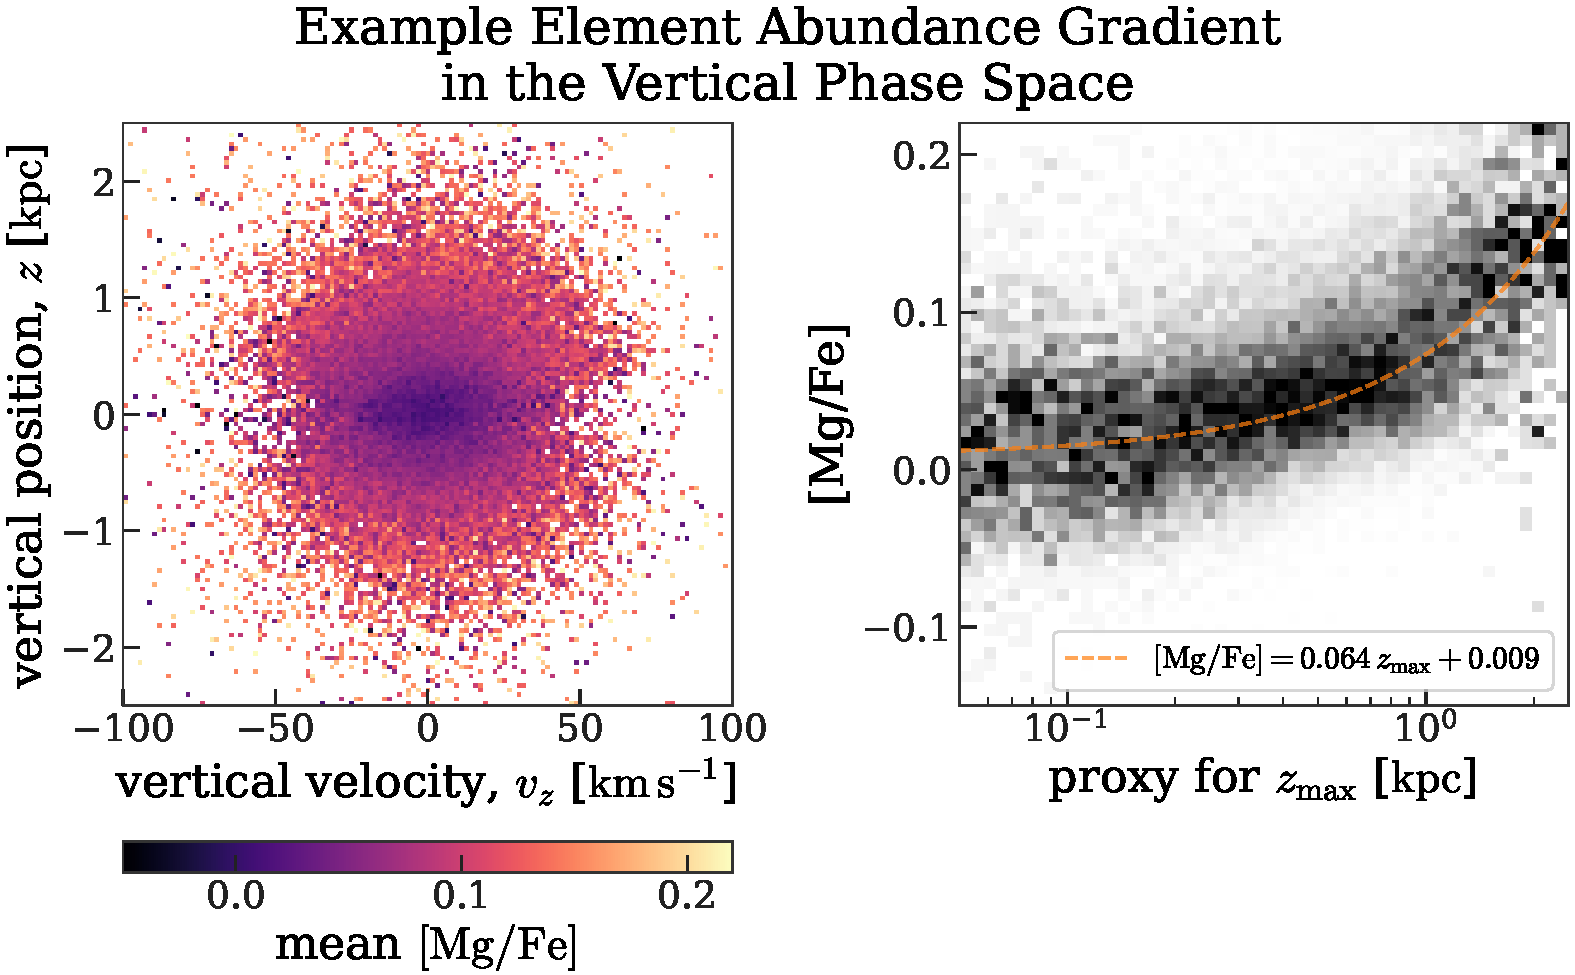
\includegraphics[width=1\textwidth]{mgfe-zvz.pdf}
\end{center}
\caption{%
A demonstration that stellar labels correlate with stellar orbits in the vertical phase
space of the Milky Way disk.
\textbf{Left panel:} Seven orbits computed in a Milky Way mass model (see
Appendix~\ref{sec:appendix-potential}) and shown in the vertical phase space, $(z,
v_z)$.
The orbits have equally-spaced values of the maximum height above the midplane each
orbit reaches, \zmax.
The vertical action, $J_z$, of these orbits scales approximately like $J_z \propto
\zmax^2$, and all orbits have $J_R=0$ and $J_\phi\approx 1900~\kms~\kpc$.
\textbf{Middle panel:} The mean \abun{Mg}{Fe} abundance for stars in the low-$\alpha$
sequence and with angular momenta $L_z$ within $\pm 15\%$ of the value for a circular
orbit at the Sun's position ($L_{z, c} \approx 1900$).
The mean \abun{Mg}{Fe} abundance is shown in small bins of the vertical position, $z$,
and velocity, $v_z$.
The mean abundance is systematically different for stars with low vertical action $J_z$
(i.e. near $(z, v_z) \sim (0, 0)$) as compared to stars with larger vertical action.
\textbf{Right panel:} The column-normalized density of stars in \abun{Mg}{Fe} as a
function of an observable proxy for $\zmax$.
We estimate a proxy for \zmax\ for the data \emph{without using a potential model} by
selecting only stars with $|v_z| < 10~\kms$ (i.e. stars that are near their vertical
apocenter).
The over-plotted dashed (orange) line shows a linear relation between \abun{Mg}{Fe} and
\zmax.
\label{fig:mgfe-zvz}
}
\end{figure*}


\section{Orbital Torus Imaging} \label{sec:oti}

The orbital actions $\bs{J}$ are useful quantities for summarizing orbits and
constructing dynamical models.
However, they require a global model for the gravitational potential, are expensive to
compute, and are not directly observable.
Fortunately, for increasingly large samples of stars in the Milky Way, we have access to
measurements of intrinsically-invariant stellar labels, such as surface element
abundance ratios or stellar ages.
These stellar labels can be used instead to trace out the orbit structure of the Galaxy.
This forms the basis of the method of Orbital Torus Imaging (OTI; \citealt{PW:2021}),
which we describe below.
Here we build on past work by developing a new framework and implementation of OTI that
leverages modern auto-differentiation tools (e.g., \jax; \citealt{jax:2018}) to
generalize and accelerate the model construction and fitting.


\subsection{Using stellar labels to map orbits}
\label{sec:oti-stat}

% TODO: mention "direct contouring" in phase-space density below -- and that the
% phase-space density itself can be a label

% From the shapes of these orbits, we can then infer the underlying acceleration field
% and therefore constrain the mass distribution of the Galaxy.
% We will also assume that, for each star, we have measurements of a set of invariant
% ``labels'' $\bs{F}$, and that those labels are correlated with the orbital properties
% of the tracers $\bs{F}(\bs{w})$, for now assuming the dependence is deterministic.

% In an equilibrium system where we have measured stellar kinematics $\bs{w} = (z, v_z)$
% and invariant labels $\bs{F}$ that appear to correlate with the orbits of stars, the
% labels can only depend on the phase-space coordinates through the vertical action
% $J_z$ or any function of the vertical action and not the vertical angle $\theta_z$.
% This comes from the assumption that the labels are invariant: If they depended on
% orbital angle $\theta_z$, this would imply that the labels change over the course of
% an orbit.

% We also then show how, with an OTI model of the orbit structure, this method can be used
% to compute empirical actions, angles, and frequencies that do not require assuming a
% global potential model.

Stars have a number of observable properties that are approximately invariant over their
lifetimes, or at least over galactic orbital timescales.
For example, the surface element abundance ratios, birth time (as a time-invariant proxy
of age), and stellar mass, to name a few.
We represent these quantities with the vector $\bs{Y}$, which we refer to as the
``stellar labels''.
In the Milky Way, these quantities are observed to correlate with the orbital
properties of stellar populations.
For example, there is a long known correlation between stellar age and velocity
dispersion \citep{Spitzer:1951, Sharma:2021}, the kinematic properties of mono-abundance
stellar populations depend on the value of the abundance \citep{Bovy:2016, Yu:2021,
Lian:2022}, and there are known gradients in element abundances and Galactic position
\citep[e.g.,][]{Shaver:1983, Maciel:1999, Eilers:2022, Lian:2023}.
Figure~\ref{fig:mgfe-zvz} shows an example of such a correlation in the vertical
kinematics of stars in the Milky Way.
The left panel of Figure~\ref{fig:mgfe-zvz} shows seven orbits in the vertical phase
space (with $J_R=0$ and $J_\phi \approx 1900~\kms~\kpc$), with equally-spaced values of
\zmax\ as computed in a Milky Way-like gravitational potential around the solar position
(see Section~\ref{sec:appendix-potential}).
The vertical action scales approximately with $J_z \propto \zmax^2$.
The middle panel shows the mean \abun{Mg}{Fe} abundance (as measured by the \apogee\
surveys, \dr{17}; \citealt{APOGEE:2017, APOGEE:DR17}) for stars in different locations
of the vertical phase space.
This demonstrates that stars with low-$J_z$ orbits (i.e. those that stay near the center
of this phase space) have systematically different element abundances than stars with
large-$J_z$ orbits (i.e. those that stay far from the center of this phase space).


% The top left panel of Figure~\ref{fig:sim-contours} shows 8 orbits with different values
% of $J_z$ (but the same values of $J_R=0$ and a $J_\phi$ similar to the solar value)
% computed in a Milky Way-like gravitational potential (see
% Section~\ref{sec:appendix-potential}).
% The orbits are colored by their vertical action, demonstrating that orbits with larger
% vertical actions cover a larger area in vertical phase space and reach higher maximum
% heights above the midplane $z_{\textrm{max}}$.
% Note that the actions define surfaces that foliate the phase space; in the case of
% vertical dynamics, the 1D curves of constant $J_z$ (i.e. the orbits) can never
% intersect.

Under the assumptions listed in Section~\ref{sec:dynreview}, the correlations between
any intrinsic, time-invariant stellar properties $\bs{Y}$ and the orbital properties of
stars can only depend on the orbital actions $\bs{J}$ and not the angles $\bs{\theta}$,
which are time dependent.
This is useful because it means we can use the stellar labels as constants of motion
themselves to trace out the shapes of orbits in phase-space.
In the context of vertical dynamics, the vertical action $J_z$ is, by construction,
constant along an orbit, so any time-invariant function of the vertical action is also
constant along an orbit.

With a suitably large sample of stars, this provides a means to measure the orbital
structure the acceleration field of the Galaxy directly, without having to assume a form
for the potential and without needing to compute the actions.
As long as the gradient in stellar labels as a function of vertical action
$\deriv{Y}{J}$ is non-zero (i.e. not flat), we can use the level sets of constant
stellar label $Y$ to ``contour'' the orbits in the vertical phase space $(z,
v_z)$.\footnote{We note that this idea, in the context of using the phase-space density
as a stellar label, was briefly discussed in \citet{Kuijken:19XX} and referred to as
``direct contouring'' of the DF.}
From the orbit contours, we can directly measure the vertical acceleration $a_z$: For
any invariant stellar label $Y$, the total time derivative $\Deriv{Y}{t}$ must be equal
to zero,
\begin{align}
    \Deriv{Y}{t} &= \pderiv{Y}{t} +
        \pderiv{Y}{z} \, \deriv{z}{t} + \pderiv{Y}{v_z} \, \deriv{v_z}{t} = 0 \\
    0 &= \pderiv{Y}{z} \, v_z + \pderiv{Y}{v_z} \, a_z
\end{align}
where $a_z = \deriv{v_z}{t}$ is the vertical acceleration.
Rearranging this expression, we can write the vertical acceleration as
\begin{align}
    a_z &= - v_z \, \pderiv{Y}{z} \left(\pderiv{Y}{v_z}\right)^{-1} \label{eq:Y-az}
\end{align}
where the right hand side and partial derivatives are evaluated along a curve of
constant $Y$.

A simple example of this is the case where the stellar label $Y$ is a function of the
vertical energy $Y=Y(E_z)$ where
\begin{equation}
    E_z = \frac{1}{2} v_z^2 + \Phi_z(z)
\end{equation}
and $\Phi_z(z)$ is the vertical potential.
In this case, the partial derivatives in Equation~\ref{eq:Y-az} are:
\begin{align}
    \pderiv{Y}{z} &= \pderiv{Y}{E_z} \, \pderiv{\Phi_z}{z}\\
    \pderiv{Y}{v_z} &= \pderiv{Y}{E_z} \, v_z
\end{align}
so that
\begin{align}
    a_z &= - v_z \, \pderiv{\Phi_z}{z} \, \pderiv{Y}{E_z} \, \left(\pderiv{Y}{E_z} \, v_z\right)^{-1} \\
    a_z &= - \pderiv{\Phi_z}{z}
\end{align}
as expected.

\begin{figure*}[t!]
\begin{center}
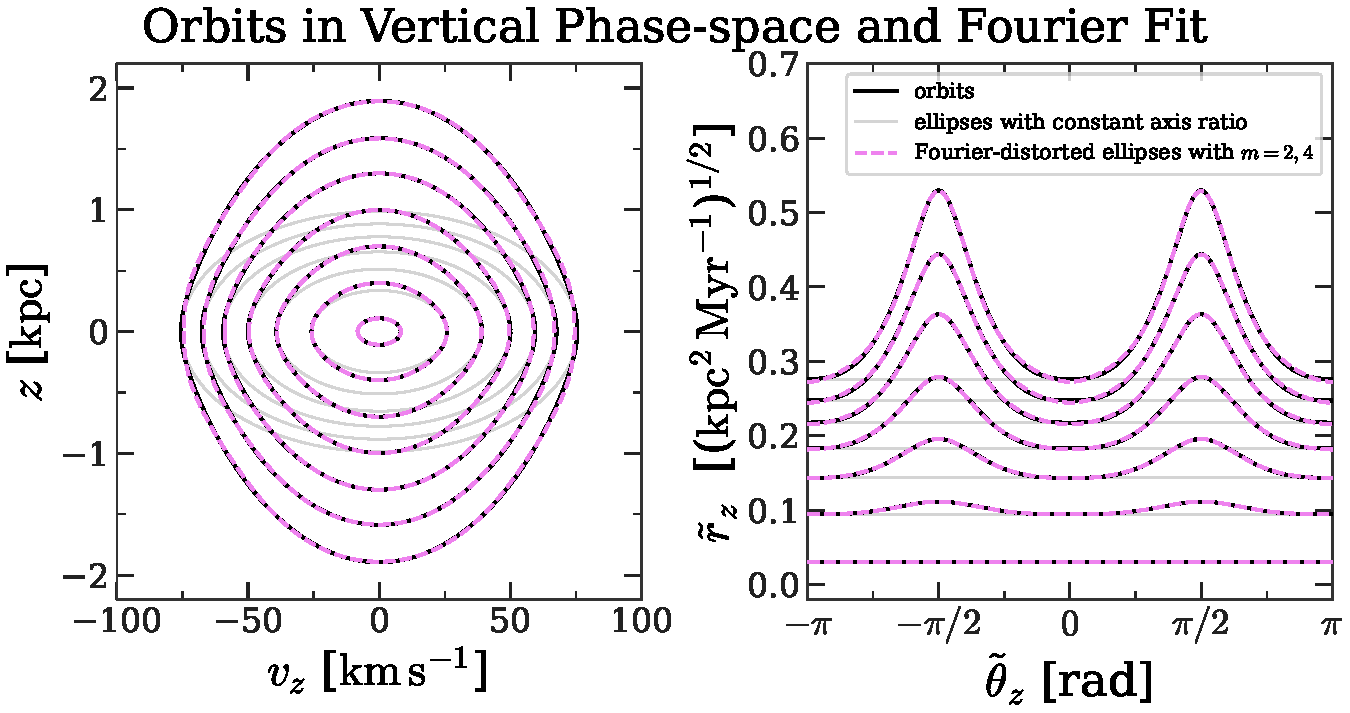
\includegraphics[width=0.8\textwidth]{simulated-orbits-fourier.pdf}
\end{center}
\caption{%
A demonstration that a low-order Fourier series expansion away from an ellipse can
represent orbit shapes in the vertical phase space of the Milky Way disk.
\textbf{Left panel:} The solid (black) lines show the same orbits as in
Figure~\ref{fig:mgfe-zvz}: These are seven orbits with equally-spaced values of the
maximum height above the midplane each orbit reaches, \zmax, computed in a mass model
for the Milky Way (see Appendix~\ref{sec:appendix-potential}).
The dashed (pink) lines show a Fourier series expansion with $m=\{2, 4\}$ with
parameters ($\rz, e_2, e_4$) determined by fitting to each orbit.
The under-plotted (gray) ellipses show ellipses with the same values of $v_{z,
\textrm{max}}$ as the orbits to emphasize that the orbits have a changing oblateness
(i.e. frequency) with increased vertical action $J_z$.
\textbf{Right panel:} The same orbits, Fourier series representations, and
constant-frequency ellipses, but now shown in the elliptical radius, \rzp\
(Equation~\ref{eq:rzp}) and angle, \thzp\ (Equation~\ref{eq:thetazp}).
\label{fig:fourier-contours}
}
\end{figure*}

Two subtleties complicate this idea.
For one, the labels are not deterministic functions of the actions.
For example, processes that cause dynamical heating of stars, which may introduce a
correlations between the vertical action, stellar age, and metallicity are inherently
stochastic \citep{TODO}.
This means that, in general, for any value of the vertical action $J_z$, there will be
a distribution of possible stellar label values.
A second complication is that we only have a finite sample of stars, so we will
never observe two or more stars on \emph{exactly} the same orbit.
Together, these necessitate working with the distribution of stellar label values
conditioned on action, $p(\bs{Y} \given J_z(z, v_z))$, such that the distribution of
stellar label values has properties or parameters that vary smoothly with the vertical
action.

In the next section, we develop a method for fitting the contours of constant stellar
label that does not assume a form for the potential $\Phi_z(z)$.
Instead of modeling the full distribution $p(\bs{Y} \given z, v_z)$, we assume that our
data are measurements of \emph{moments} of the distribution at different locations in
phase-space.
Contours of constant moments of the stellar label distribution equivalently satisfy the
expressions above (e.g., Equation~\ref{eq:Y-az}).
For example, the mean value of a stellar label $\mean{Y}$ is
\begin{equation}
    \mean{Y} = \int \dd Y \, Y \, p(Y \given J_z) \quad .
\end{equation}
It is straightforward to show that this also satisfies $\Deriv{\mean{Y}}{t} = 0$, along
with other moments of this distribution.


% - But: f(z, vz) = C define contours
%     - fit contours, can take derivatives
%     - Another benefit: contours are orbits, so can derive actions, angles, etc.
%     - Method called "direct contouring" by (KG paper 1)
% - <Explain our way of fitting shape of contours>

% The framework described in Section~\ref{sec:vertical} is a standard approach to modeling
% the vertical kinematics of tracers in the Milky Way disk to measure properties of the
% mass distribution, like the vertical acceleration or surface mass density.
% Here we describe an alternative approach, built off of the idea of Orbital Torus Imaging
% \citep[OTI;][]{Price-Whelan:2021}.
% OTI is the idea that, in an equilibrium system, any function of the phase-space
% coordinates that ``labels'' the orbits (e.g., the orbital actions or any function of
% the actions) can be used to constrain the shapes of contours of the DF.
% This is useful because the shapes of these contours are directly related to the
% acceleration (and therefore mass distribution) through the CBE
% (Equation~\ref{eq:cbe-1d}).
% In a system with one degree of freedom, these contours are closed curves in phase-space
% that also correspond to orbital trajectories.
% In what follows, we start by considering the case of using the phase-space density or
% the value of the DF itself to fit these contours.
% We then discuss how this generalizes to using stellar label data, which we assume are
% only functions of the orbital actions and not of orbital phase (i.e. conjugate angle).
% We finally show how, in the vertical phase-space, a fitted OTI model can be used to
% compute empirical values of dynamical quantities like the orbital actions, frequencies,
% and angles.

% A core motivation for OTI is that the derivatives of the DF that appear in the CBE
% (e.g., Equation~\ref{eq:cbe-1d}) only depend on the shapes of the curves defined by
% level sets of the DF (i.e. curves of constant phase-space density), or of any
% functions of the phase-space density that depend on auxiliary data (e.g., element
% abundance ratios or other stellar labels). In a system with one degree of freedom,
% these level sets are closed curves in phase-space that also correspond to orbits. We
% start by considering the case of using the phase-space density or the value of the DF
% itself, then discuss how this generalizes to using stellar label data, and then
% finally show how, in the vertical phase-space, a fitted OTI model can be used to
% compute empirical values of dynamical quantities like the orbital actions and
% frequencies.

\subsection{A Flexible Model of Stellar Label Moments in Phase Space}
\label{sec:oti-fourier}

In this section, we develop a method to fit the shapes of contours of constant stellar
label moments in the vertical phase space of the Milky Way disk.
An example of the type of data we would like to model is shown in the middle panel of
Figure~\ref{fig:mgfe-zvz}, which shows the mean \abun{Mg}{Fe} abundances of stars in
bins of vertical phase-space coordinates for stars on near-circular orbits in the solar
neighborhood.
As we showed in the previous section (Section~\ref{sec:oti-stat}), these contours of
observed mean \abun{Mg}{Fe} abundance (or any moments of stellar labels) correspond to
orbital trajectories, under the assumptions adopted above.
To parametrize the shapes of the contours of constant stellar label, we use a Fourier
expansion away from an elliptical radius in the vertical phase space, as described
below.

As mentioned above (Section~\ref{sec:dynreview}), orbits near the Galactic midplane ($z
\approx 0$) feel an approximately uniform mass density, $\rho(z) \approx \rho_0$.
This implies that the vertical gravitational potential near the midplane will be close
to a harmonic oscillator potential in which orbits have a constant vertical frequency
$\freqzero$ (Equation~\ref{eq:freqzero}).
These orbits therefore trace closed ellipses of constant elliptical radius \rzp\ defined
as
\begin{equation}
    \rzp = \sqrt{z^2 \, \freqzero + v_z^2 \, \freqzero^{-1}} \label{eq:rzp}
\end{equation}
for all values of the corresponding ellipsoidal angle \thzp,
\begin{equation}
    \tan (\thzp) = \left(\frac{z}{v_z}\right) \, \freqzero \quad .
    \label{eq:thetazp}
\end{equation}
% where $z_0$ and $v_{z,0}$ are the midplane position and velocity, respectively.

Away from the midplane, the shapes of orbits have steadily decreasing frequencies with
increasing maximum height $z_{\textrm{max}}$, which leads to, to first order, a changing
aspect ratio of the contours.
For example, the orbits in the left panel of Figure~\ref{fig:mgfe-zvz} start oblate for
the lowest values of \zmax\ and become more prolate for the largest values of \zmax.
For contours with sufficiently large $z_{\textrm{max}}$ values (i.e. orbits that reach
many scale heights above the disk), the influence of the dark matter halo's potential
distorts the orbit shapes, and the contours of the DF are no longer well-approximated by
ellipses (e.g., the orbits with $\zmax \gtrsim 1~\kpc$ in Figure~\ref{fig:mgfe-zvz}).
The halo potential causes the orbits to deform from ellipses to more ``diamond-like''
shapes.

To represent more general contour shapes (i.e. beyond ellipses), we use a low-order
Fourier expansion in the ellipsoidal angle \thzp\ to distort the ellipsoidal radius
\rzp\ into the distorted ellipsoidal radius \rz, defined as
\begin{equation}
    \rz = \rzp \, \left[1 + \sum_m \epsilon_m(\rzp) \, \cos{\left(m\,\thzp\right)}\right] \label{eq:rz}
\end{equation}
where, for the vertical kinematics, we only consider even $m$ values to preserve the
symmetry of the contour shapes.
The functions $\epsilon_m(\rzp)$ describe the radius-dependent amplitude of the Fourier
terms, which we require to be zero at $\rzp=0$, and the values are typically $\ll 1$
for the orbits we consider (i.e. with $\zmax \lesssim 2~\kpc$ or so).
This expansion is motivated by the fact that we expect to need just a few Fourier terms:
an $m=2$ distortion with an amplitude that varies with \rzp\ will change the aspect
ratio of the elliptical contours as a function of \rzp, which acts like a changing
frequency as a function of $z_{\textrm{max}}$.
An $m=4$ distortion can ``pinch'' the contour shapes to make then more diamond-like,
which mimics the effect of an orbit feeling the halo potential.
Figure~\ref{fig:fourier-contours} shows the same orbits as in the left panel of
Figure~\ref{fig:mgfe-zvz} (solid black lines) along with a low-order Fourier expansion
fit to these orbits (dashed pink lines), showing that even with just $m=\{2, 4\}$
Fourier terms, we can accurately model the shapes of the orbits.
The left panel of Figure~\ref{fig:fourier-contours} shows the orbits and Fourier fits in
the vertical phase space, and the right panel shows the same orbits and Fourier fits in
the elliptical radius and angle coordinates, \rzp\ and \thzp.

When fitting stellar label data, we assume that the contours of constant stellar label
are only functions of the distorted radius, \rz\ (Equation~\ref{eq:rz}).
This then enforces that \rz\ is constant along a contour of constant label value and,
therefore, nearly constant along a vertical orbit.
We then need to specify a functional form for the dependence of the stellar label moment
on \rz, $Y(\rz)$, which we assume is a smooth function of \rz\ but is otherwise
customizable (we adopt choices below in the demonstrations in
Sections~\ref{sec:applications-sim}--\ref{sec:applications-data}).
The model components that must be specified in order to fit this model given a sample of
stellar phase-space positions and labels are: the Fourier distortion amplitude functions
$\epsilon_m(\rzp)$ for all $m$ orders up to the specified \mmax, the functional form and
any parameters of the stellar label function $Y(\rz)$, and the asymptotic midplane
orbital frequency \freqzero.
As we will be fitting this model to data where we do not know the true zero-point
position or velocity of the midplane, we additionally include parameters $z_0$ and
$v_{z,0}$ to represent these zero-point values --- we then replace $z$ and $v_z$ in
Equations~\ref{eq:rzp}--\ref{eq:thetazp} with $z-z_0$ and $v_z - v_{z, 0}$.

As the label function only depends on the distorted radius \rz, we can compute the
vertical acceleration from a fitted OTI model directly from the dependence of \rz\ on
the phase space coordinates.
That is, from Equation~\ref{eq:Y-az} and applying the chain rule, we have
\begin{equation}
    a_z = - v_z \, \pderiv{r_z}{z} \left(\pderiv{r_z}{v_z}\right)^{-1} \quad .
\end{equation}
From the definition of \rz\ and after some manipulation (see
Appendix~\ref{sec:appendix-az}), we find that
\begin{equation}
    a_z(z) = - \freqzero^2 \, z \,
    \frac{\left[
        1 + \sum_{j=1}^{\mmax/2} (-1)^{j} \,
            \left(e_m + \rzp \, \frac{\partial e_m}{\partial \rzp}\right)
    \right]_{\rzp = \sqrt{\freqzero}\,z}}{\left[
        1 + \sum_{j=1}^{\mmax/2} (-1)^{j} \,
            \left(e_m\,(1 - m^2) + \rzp \, \frac{\partial e_m}{\partial \rzp}\right)
    \right]_{\rzp = \sqrt{\freqzero}\,z}} \label{eq:az-ugly}
\end{equation}
where $m=2\,j$ and $\mmax$ is the maximum (even) order of the Fourier expansion of the
distorted radius, and the expression is evaluated at $\rzp = \sqrt{\freqzero}\,z$.
Note that when $e_m = 0$ for all $m$ (i.e. when there is no distortion of the
ellipsoidal radius), this reduces to the expected expression for the simple harmonic
oscillator.

We obtain the expression above for $a_z(z)$ (Equation~\ref{eq:az-ugly}) by taking the
limit $\thzp \rightarrow \pi/2$, which, in our definition, is equivalent to the limit
$v_z \rightarrow 0$.
However, because our model parametrizes the shapes of orbits without imposing
physicality, our inferred force law can end up depending on velocity.
This is unphysical, but is a tradeoff we make to allow for a flexible model of the phase
space --- we discuss this point further in the Discussion
(Section~\ref{sec:discussion-vz-dependence}).
Another potential pathology of our model setup is that, for some settings of the
functions $e_m(\rzp)$, the orbits can cross (i.e. the contours of constant label can
intersect).
In a truly separable system, this would also lead to unphysical interpretations of the
force field inferred from the model, as the orbits should foliate the phase space.
We do not find this to be a problem in practice with sufficient bounds set on the
Fourier distortion functions to keep their amplitudes small.
% \todo{words about drz/drzp, foliation, non-overlapping contours}

We have implemented this new Orbital Torus Imaging (OTI) framework in \python\ using
\jax\ \citep{jax:2018} to accelerate the model evaluation and to use automatic
differentiation to compute the gradients of the model with respect to the (many) model
parameters.
We release a software package, \texttt{torusimaging}, along with this Article that
contains our implementation.
This framework is therefore very general and our implementation accepts any functional
forms for the model components.


\subsection{Computing empirical actions and angles}
\label{sec:empirical-aaf}

The distorted elliptical radius \rz\ will be close to constant along orbits in the
vertical phase space.
The orbital action and frequency should therefore be monotonic and smooth functions of
\rz, i.e. $J_z = J_z(\rz)$ and $\Omega_z = \Omega_z(\rz)$.
We can therefore use a fitted model of the contours of constant stellar label to compute
empirical values of the action, conjugate angle, and frequency for a given phase-space
position $(z, v_z)^*$.
We compute these dynamical quantities using the integrals in
Equations~\ref{eq:Jz}--\ref{eq:Tz} by integrating over the ellipsoidal angle $\thzp$
along a contour of constant $\rz$:
\begin{align}
    J_z &= \frac{2}{\pi} \, \int_0^{\pi/2} \dd \thzp \, v_z(\thzp)
        \, \left|\frac{\dd z}{\dd \thzp}\right| \label{eq:Jz-ell} \\
    T_z &= 4 \, \int_0^{\pi/2} \frac{\dd \thzp}{v_z(\thzp)}
        \, \left|\frac{\dd z}{\dd \thzp}\right| \label{eq:Tz-ell}
\end{align}
where the function $v_z(\thzp)$ and the Jacobian term $\left|\frac{\dd z}{\dd
\thzp}\right|$ are evaluated along a curve of constant $\rz$ corresponding to the
phase-space coordinates $(z, v_z)^*$.
The conjugate angle variable, $\theta_z$, is computed as the fractional time
\begin{equation}
    \theta_z = \frac{2\pi}{T_z} \, \int_0^{\thzp^*} \frac{\dd \thzp}{v_z(\thzp)}
        \, \left|\frac{\dd z}{\dd \thzp}\right| \label{eq:thz-ell} \quad .
\end{equation}

\section{Applications to Simulated Data} \label{sec:applications-sim}

% TODO: decide on a policy for deciding maximum z, vz (i.e. 95th percentile values or
% something??) and use that for all examples

In this section, we demonstrate the OTI framework described above using a set of
simulated datasets of increasing complexity.
We start by using a one-dimensional simple harmonic oscillator potential
(Section~\ref{sec:sim-sho}), then use a more realistic multi-component (3D) galaxy model
(Section~\ref{sec:sim-qiso}--\ref{sec:sim-qiso-sel}), and finally use the final snapshot
from an $N$-body simulation of a disk galaxy perturbed by an orbiting satellite
(Section~\ref{sec:sim-jason}).
As input to OTI, we bin the data into pixels of vertical position $z$ and velocity $v_z$
and compute the mean abundance value in each pixel, but we do not simulate uncertainties
on the phase-space coordinates.
We set the maximum bin edge in each coordinate as three times the 90th percentile value
of the distributions of $z$ and $v_z$ for each simulated sample, and use 151 bins for
each coordinate.
These choices are arbitrary, but we have verified that the results are not sensitive to
reasonable changes of these values.
In the following subsections, we demonstrate that OTI can recover the true vertical
acceleration profiles and other dynamical quantities for these simulated data sets.

% For our implementation used in this article, we adopt the following:
% \begin{align}
%     m &= \left\{2, 4\right\} \\
%     e_2(r_z') &\geq 0 \,\,\forall r_z'\\
%     e_4(r_z') &\leq 0 \,\,\forall r_z'
% \end{align}
% and we use linear splines to represent the functions $n(r_z)$, $e_2(r_z')$, and
% $e_4(r_z')$.

\subsection{Simple Harmonic Oscillator}
\label{sec:sim-sho}

As an initial application, we simulate phase-space data in a harmonic oscillator
potential,
\begin{equation}
    \Phi_{z}(z) = \frac{1}{2} \, \omega^2 \, z^2
\end{equation}
by sampling from an isothermal distribution function\footnote{We will use $f(\cdot)$ to
represent a distribution function, \df, that integrates to a number of stars, and
$p(\cdot)$ to represent a normalized \df\ that integrates to 1 (i.e. a probability
distribution function).}
\begin{align}
    p_z(J_z) &= \frac{1}{\, s_z} e^{-\frac{J_z}{s_z}} \quad ; \quad J_z \in [0, \infty)\\
    s_z &= \sigma_{v_z}^2 / \omega\\
    z = \sqrt{\frac{2 \, J_z}{\omega}} \, \sin\theta_z \quad &; \quad
        v_z = \sqrt{2 \, J_z \, \omega} \, \cos\theta_z
\end{align}
We adopt $\omega = 0.08~\unit{\radian\per\mega\year}$ and $\sigma_{v_z} = 50~\kms$ as
somewhat arbitrary choices meant to approximately match the observed vertical kinematics
of stars near the solar position.
We sample $N=2^{18}=\num{262144}$ phase-space positions to use as our simulated data
set, but we note that the precision of our measurements (especially at high $z$) will
depend on the sample size.
We then assign each star a simulated element abundance value to serve as a stellar label
$Y$: We use the relation between \abun{Mg}{Fe} and $z_{\textrm{max}}$ from the \apogee\
data (see the right panel of Figure~\ref{fig:mgfe-zvz}) to assign each star a simulated
value of $Y_{\abun{Mg}{Fe}}$ by drawing from a Gaussian centered on the mean value from
the linear relation with a standard deviation of $0.05~\textrm{dex}$.
That is, our simulated abundance values are drawn from
\begin{equation}
    Y_{\abun{Mg}{Fe}} \sim \mathcal{N}(0.064~\zmax + 0.009, 0.05)
\end{equation}
where $\mathcal{N}(\mu, \sigma)$ is a normal distribution with mean $\mu$ and standard
deviation $\sigma$.
We then additionally simulate measurement errors on the abundance values by drawing an
abundance uncertainty, $\sigma_Y$, for each star particle such that $\log \sigma_Y \sim
\mathcal{U}(-4, 0.5)$, where $\log$ is the natural logarithm and $\mathcal{U}(a, b)$ is
the uniform distribution over the domain $[a, b)$.
Figure~\ref{fig:sho-data-model} (left panel) shows the mean simulated \abun{Mg}{Fe}
abundance for stars in bins of vertical phase-space coordinates with the same color
scale as in the middle panel of Figure~\ref{fig:mgfe-zvz} (i.e. the real \apogee\ data).

\begin{figure*}[t!]
\begin{center}
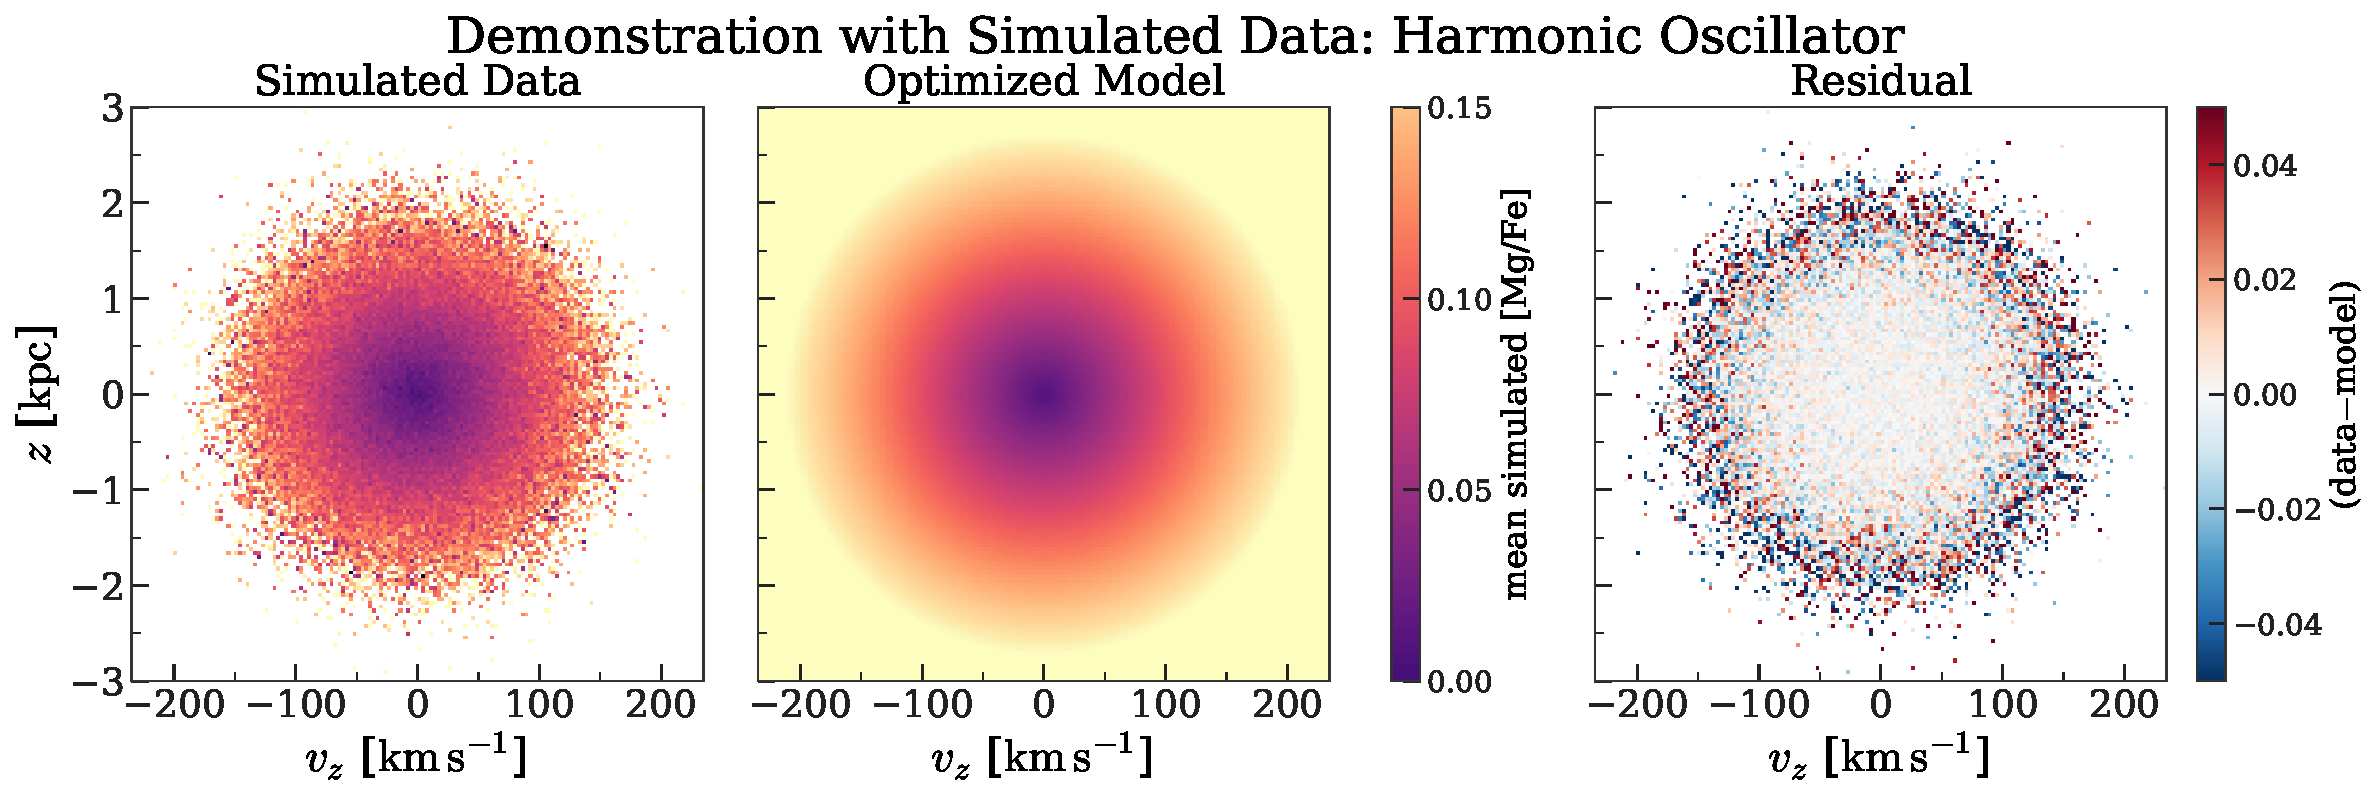
\includegraphics[width=\textwidth]{sho-data-model.pdf}
\end{center}
\caption{%
A demonstration of an optimized OTI model using simulated data in a simple harmonic
oscillator potential.
\textbf{Left panel:} Simulated kinematic data in the vertical phase space with an
isothermal distribution function and a linear relation between \abun{Mg}{Fe} and
$z_{\textrm{max}}$ (see Figure~\ref{fig:mgfe-zvz}).
\textbf{Middle panel:} The optimized OTI model evaluated on the same grid of phase-space
coordinates as the data (left panel).
\textbf{Right panel:} The residuals of the optimized model (i.e. the simulated data
minus the optimized model, evaluated on the same grid of phase-space coordinates).
The small residuals (except on the edges, where the number of stars per pixel is small) show that the model accurately represents the mean abundance trends in this phase space.
\label{fig:sho-data-model}
}
\end{figure*}

We then fit the simulated mean abundance data in pixels of phase-space coordinates,
$\langle Y_{\abun{Mg}{Fe}} \rangle$, using the OTI framework described above
(Section~\ref{sec:oti}).
To do this, we need to decide on functional forms for both the label function, $Y(\rz)$,
and the Fourier coefficient functions.
For all of these functions, we use monotonic quadratic spline functions defined such
that the function is always monotonically increasing or decreasing, which must be
hard-set before optimization (see Appendix~\ref{sec:appendix-spline}).
For the label function, we assert that the value must monotonically increase from $\rz =
0$ to the maximum spline knot location.
We use $K_Y=10$ spline knot locations $x_k^{(Y)}$ equally spaced in $\rz$ between $0$
and $r_{z, \textrm{max}}$ with function values at the knot locations $y_k^{(Y)}$.

For this initial test case, we include only an $m=2$ term in our Fourier distortion of
the elliptical radius (Equation~\ref{eq:rz}).
For the Fourier coefficient function, $e_2(\rzp)$, we require that the coefficient value
must equal zero at $\rzp = 0$ (i.e. $e_2(0) = 0$), and that the coefficient value
monotonically increases with $\rzp$.
Requiring $e_2(0) = 0$ ensures that the parameter $\freqzero$ corresponds to the
asymptotic orbital frequency as $\rzp \rightarrow 0$ and can therefore be used to
estimate the midplane volume mass density (Equation~\ref{eq:freqzero}).
Assuming that the coefficient value increases with $\rzp$ (so that the orbit shapes
can only become more prolate with increasing $z_{\textrm{max}}$) is equivalent to
assuming that the surface density increases with increasing height $z$.
We use $K_e=5$ spline knot locations $x_k^{(e_2)}$ with values $y_k^{(e_2)}$ equally
spaced in $\rz$ between $0$ and $r_{z, \textrm{max}}$, but we require the knot value at
$\rzp = 0$ to be equal to zero $y_0^{(e_2)}=0$.
All of the parameters used in this demonstrative model fit and the adopted bounds used
when optimizing are summarized in Table~\ref{tbl:sho-params}.
When optimizing, we reparameterize to use $\log \freqzero$ and $\log y_k$ for any spline
coefficients to control the sign of the parameter values.

Our framework is implemented with \jax\ so that our objective function is just-in-time
compiled and we can use automatic differentiation to compute the gradients of the
objective function with respect to the, in this case, 17 model parameters.
We use a Gaussian log-likelihood for the mean \abun{Mg}{Fe} abundance data as our
objective function.
For the uncertainty on the mean abundance in each pixel, we consider both the error on
the mean (given heteroskedastic measurement errors on the abundances of each star
particle, $\sigma_{Y,i}$),
\begin{equation}
    \sigma_{\mu_Y} = \sqrt{\frac{1}{\sum_i \frac{1}{\sigma^2_{Y,i}}}}
\end{equation}
and the intrinsic scatter of abundances in each pixel.
We assume for this case that we do not know the true intrinsic scatter that we simulated
with in order to emulate working with real data, so we compute the error-deconvolved
intrinsic scatter, $s_y$, of abundance values in the ten pixels with the most number of
star particles.
We take the uncertainty of the mean abundance $\mu_{Y,j}$ in each pixel $j$ to be
\begin{equation}
    \sigma_{\mu_{Y,j}} = \sqrt{\sigma_{\mu_Y, j}^2 + s_Y^2 / N_j}
\end{equation}
where $N_j$ is the number of star particles in pixel $j$ and $\sigma_{\mu_Y, j}$ is the
error on the mean in the same pixel.

We additionally use an L2 regularization on the Fourier coefficient function values
$y^{(e_2)}$ with a standard deviation of 0.1, and on the label function spline values
$y^{(Y)}$ with a standard deviation of 1, to try to keep these values near zero when the
data are uninformative.
We use a standard L-BFGS-B optimizer \citep{Byrd:1995} to minimize the regularized
negative log-likelihood, implemented in \texttt{JAXopt} \cite{jaxopt:2021}.
For this simulated data, the optimization runs in $\sim 10~\unit{\second}$ on a single
CPU.
The middle panel of Figure~\ref{fig:sho-data-model} shows the best-fit model evaluated
over the domain of our simulated data in the left panel, and the right panel shows the
residuals.
The residuals everywhere indicate that the best-fit model matches the data well.

We use the optimized parameter values to initialize two Markov Chain Monte Carlo (MCMC)
chains using the Hamiltonian Monte Carlo ``No U-turn Sampler'' (NUTS) implemented in the
\texttt{blackjax} \citep{blackjax} Python package.
We run the chains for 1000 initial steps to allow the NUTS sampler to tune the
hyperparameters of the sampling procedure (e.g., the mass matrix), and then run for an
additional 1000 steps.
The left panel of Figure~\ref{fig:sho-validation} shows the maximum a posteriori (MAP)
vertical acceleration profile, $a_z(z)$ (computed with Equation~\ref{eq:az-ugly}), as
the under-plotted black line, and the over-plotted, dashed (green) line shows the true
vertical acceleration relation, $a_z = -\omega^2 \, z$.
This demonstrates that, for this toy dataset, we are able to recover the true
acceleration profile using OTI.
In the same panel, we also plot a shaded (gray) polygon to represent the acceleration
profile span for the 16th--84th percentile values of the MCMC samples.
However, in this case, the uncertainty region is comparable to the thickness of the
black line.

The middle panel of Figure~\ref{fig:sho-validation} shows eight orbits with
equally-spaced (but arbitrary) values of the vertical velocity at $z=0$: The
under-plotted solid (black) lines show the orbital trajectories inferred using the MAP
parameter values with our OTI model, and the over-plotted dashed (green) lines show the
true orbital trajectories for this toy model, demonstrating agreement.
The right panel of Figure~\ref{fig:sho-validation} shows the true vertical action values
for all simulated particles on the vertical axis (i.e. the samples from the \df\ used to
create the mean abundance data shown in the left panel of
Figure~\ref{fig:sho-data-model}) and our estimates for the vertical action of each star
particle as the black point markers, computed using the MAP parameter values.
We compute the actions, frequencies, and angles using
Equations~\ref{eq:Jz-ell}--\ref{eq:thz-ell} evaluated at the phase-space coordinates of
each star particle.
The acceleration error at $z=1~\kpc$ is $< 1\%$ (in fractional error) and the median
action error is $<0.5\%$ for this toy dataset.

\begin{figure*}[t!]
\begin{center}
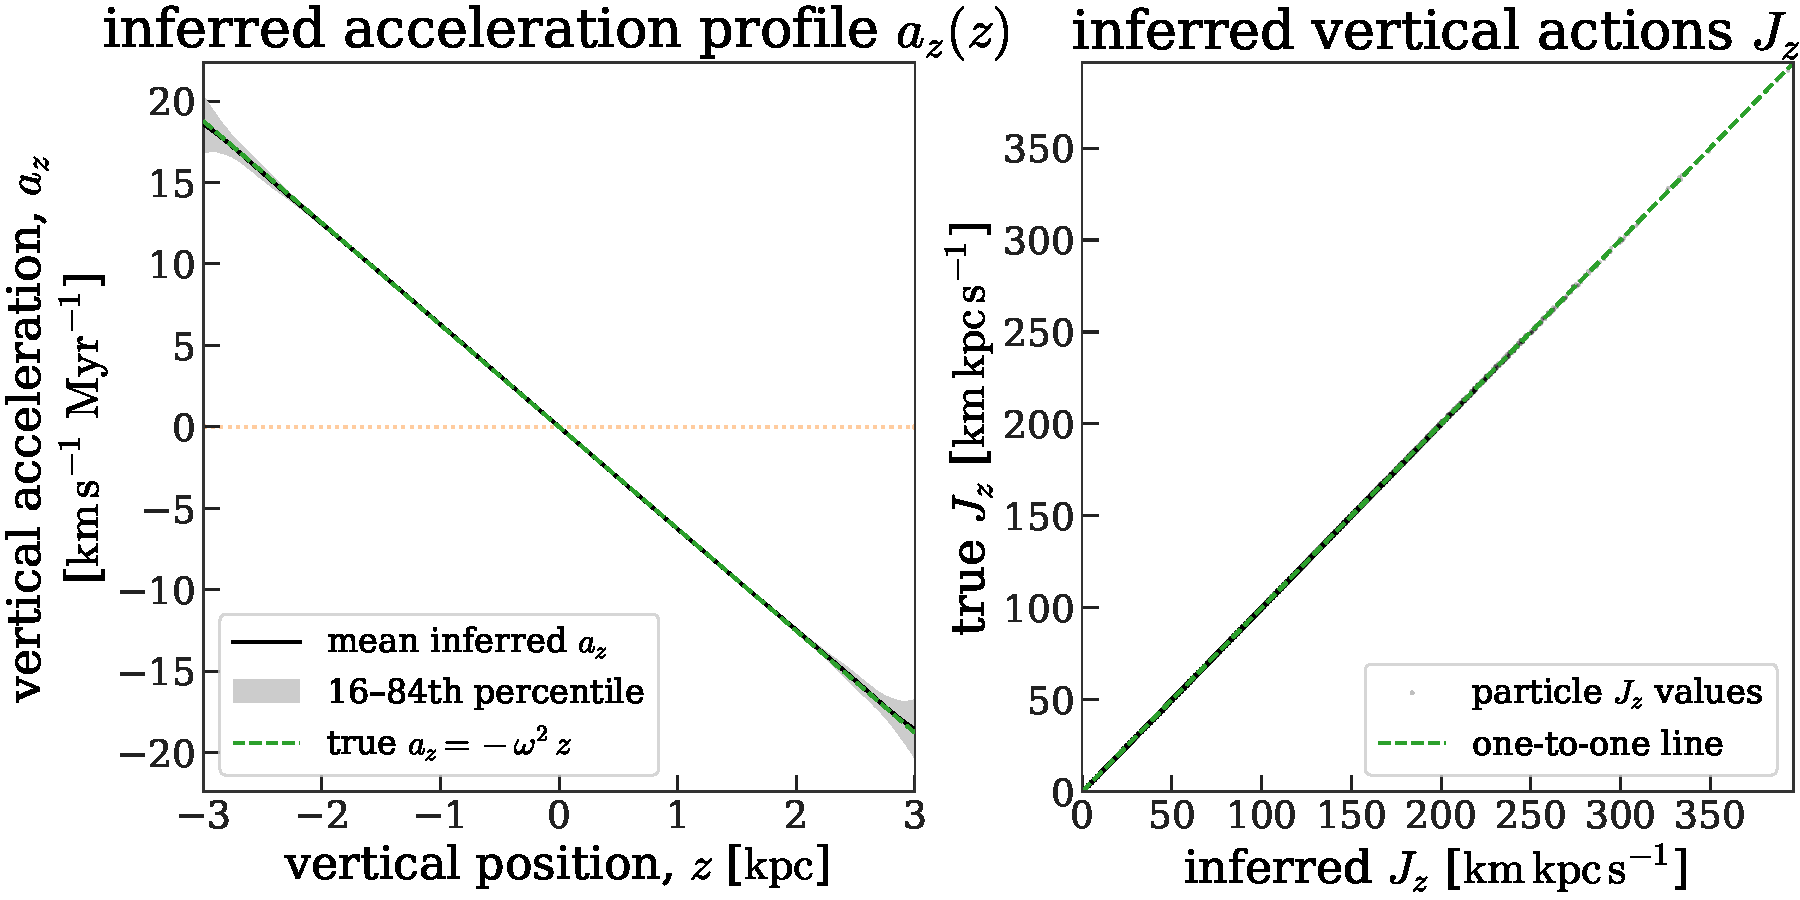
\includegraphics[width=\textwidth]{sho-validation.pdf}
\end{center}
\caption{%
\todo{suptitle same as previous figure?}
Validation of the OTI model fit to the simulated simple harmonic oscillator data.
\textbf{Left panel:} The inferred (maximum a posteriori; MAP) vertical acceleration
profile, $a_z(z)$, from the OTI model (solid black line) compared to the true
acceleration profile (dashed green line).
The uncertainty in the acceleration trend is comparable to the width of the line.
Most of the simulated data are within $|z| \lesssim 2~\kpc$ and the inferred
acceleration profile agrees well with the true values within this region.
\textbf{Middle panel:} Eight orbits with equally-spaced values of the vertical velocity
computed in the true potential model (simple harmonic oscillator; shown as dashed, green
lines) and with the OTI model using the MAP parameter values (solid, black lines).
\textbf{Right panel:} A comparison of the true vertical action values (vertical axis)
and our estimates using the MAP OTI model (horizontal axis).
Our action estimates are empirical in that we do not need to assume the form for a
gravitational potential.
The median (fractional) action error is $<0.5\%$ for this sample dataset.
\label{fig:sho-validation}
}
\end{figure*}

\subsection{Axisymmetric Quasi-isothermal Disk}
\label{sec:sim-qiso}

As a next application of the OTI framework, we use a more realistic galaxy model to
sample 3D positions and velocities of star particles to test our inferred quantities in
a more realistic setting.
We use a quasi-isothermal disk distribution function \citep[\df;][]{Binney:2012} with
parameters derived from fitting Milky Way stellar data (we use the ``thin disk''
parameters from Table~3 of \citealt{Sanders:2015}).
We implement this \df\ using the \agama\ package and sample \num{5d8} phase-space
coordinates with guiding-center radii $R_G$ between $5 < R_G < 12~\kpc$ embedded in our
adopted Milky Way potential model (see Appendix~\ref{sec:appendix-potential}).
We compute the guiding radii using an approximation assuming the circular velocity
curve, $v_c(R)$, is flat, $R_G = L_z / v_c(R)$, where $L_z$ is the angular momentum of
the star particle and $R$ is its instantaneous cylindrical radius.
From this simulated sample, we select only stars near the solar radius, $R_0=8.3~\kpc$,
with $|R-R_0| < 1~\kpc$, and additionally select $|R-R_G| < 1~\kpc$ and $|v_R| <
15~\kms$ as a way of limiting the radial action of the stars so that our assumption of
$R$--$z$ separability is more valid.
We do not use the radial action itself to select stars because we want to mimic the
kinds of selections we could do with real data, where we do not know the true underlying
gravitational potential (which would be needed to compute the actions).
After these selections, we are left with $\approx \num{7d6}$ star particles.
We again compute simulated \abun{Mg}{Fe} abundance values for these stars using the
linear relation between \abun{Mg}{Fe} and $z_{\textrm{max}}$ from the \apogee\ data (see
the right panel of Figure~\ref{fig:mgfe-zvz}) and a scatter of 0.05~dex (see
Section~\ref{sec:sim-sho}), with simulated uncertainties following
Section~\ref{sec:sim-sho}.
The left panel of Figure~\ref{fig:qiso-data-model} shows this simulated data set in the
vertical phase space coordinates.

We fit the simulated mean abundance data in pixels of phase-space coordinates using the
OTI framework described above (Section~\ref{sec:oti}) and following the same procedure
as in Section~\ref{sec:sim-sho}.
We again use monotonic quadratic spline functions (Appendix~\ref{sec:appendix-spline})
for both the label function and the Fourier coefficient functions.
For the label function, we use 8 knots equally spaced in \rz\ between $0$ and $r_{z,
\textrm{max}} \approx 0.53~\unit{\kilo\parsec\per\mega\year\tothe{1/2}}$.\todo{update}
However, here we use $m=\{2, 4\}$ Fourier terms with 8 and 4 spline knots, respectively.
We space the Fourier coefficient spline knots equally in $\rz^{3/2}$ between $0$ and
$r_{z, \textrm{max}}$: This places a higher density of knots at lower \rz\ values where
we expect the Fourier coefficient functions to change more rapidly.
We again require that the coefficient function values are zero at $\rzp = 0$ so that
$e_2(0)=e_4(0)=0$, and we assume that the overall sign of the functions are $(+,-)$ for
the $m=\{2, 4\}$ coefficient functions, respectively.

We use the same regularization as in Section~\ref{sec:sim-sho} (L2 regularization on the
coefficient function parameters with a standard deviation of 0.1 and on the label
function parameters with a standard deviation of 1) for all Fourier coefficient
functions.
As above, we initially use a L-BFGS-B optimizer to minimize the regularized negative
log-likelihood.
This model has 22 parameters and optimizes in $\sim 30$~seconds on a single CPU.
The middle panel of Figure~\ref{fig:qiso-data-model} shows the best-fit model evaluated
on the same pixel grid as the simulated data, and the right panel shows the residuals
between the optimized model and the data, normalized by the uncertainty on the mean
abundance in each pixel.
The small residuals indicate that this model does well to fit the mean abundance
variations in the vertical phase space.

We again use the optimized parameter values to initialize an MCMC sampling of the
parameters following the same procedure as in Section~\ref{sec:sim-sho}.
The left panel of Figure~\ref{fig:qiso-validation} shows the inferred vertical
acceleration profile (black line; computed with the MAP parameter values) and
uncertainties (gray shaded region; computed using the 16th--84th percentile parameter
values using the MCMC samples) along with the true vertical acceleration (green dashed
line) evaluated at a constant $R=R_0$ in our adopted Milky Way potential model (see
Appendix~\ref{sec:appendix-potential}).
The acceleration precision at $z=1~\kpc$ is $\sim 1\%$ (in fractional error) with a
$\sim 1\%$ bias.

The middle panel of Figure~\ref{fig:qiso-validation} shows eight orbits with
equally-spaced (but arbitrary) values of the vertical velocity at $z=0$: The
under-plotted solid (black) lines show the orbital trajectories inferred using the MAP
parameter values with our OTI model, and the over-plotted dashed (green) lines show the
true orbital trajectories.
The true orbital trajectories are computed in the 3D galaxy model using the grid of
$v_z$ values at $z=0$ with $x=R_0$, $v_x=0$, and $y=0$.
To set $v_y$ for the true orbits, we take the true actions computed for the particles in
our selected region and fit a 3rd-order polynomial to the relationship between $J_\phi$
and $J_z$ in this region (which arises primarily because of the finite selection on
$R$).
For the grid of $v_z$ values, we transform to $J_z$ and evaluate the fitted polynomial
to obtain a $J_phi$ value, which we then convert to $v_y$ by dividing out the radius
$R_0$.
There is good agreement between the true and inferred acceleration profile and orbits,
especially for $|z| \lesssim 1~\kpc$.
Above $|z| \gtrsim 1~\kpc$, the true orbit shapes and the OTI-inferred orbits begin to
defer as the assumption of $R$--$z$ separability becomes less and less applicable.

We again compute the actions, frequencies, and angles for the star particles using
Equations~\ref{eq:Jz-ell}--\ref{eq:thz-ell} evaluated at the phase-space coordinates of
star particles in this simulated data set.
The right panel of Figure~\ref{fig:qiso-validation} shows (as black markers) the true
vertical action values for a random subset of $10^5$ simulated particles on the vertical
axis and our estimates for the vertical action of each star particle using the OTI
model.
We find the median fractional error of the vertical action, angle, and frequency are
$\sim 5\%$, $\sim 5\%$, and $\sim 9\%$, respectively. \todo{Compute all numbers again,
and do for 100,000 not 20,000}


\begin{figure*}[t!]
\begin{center}
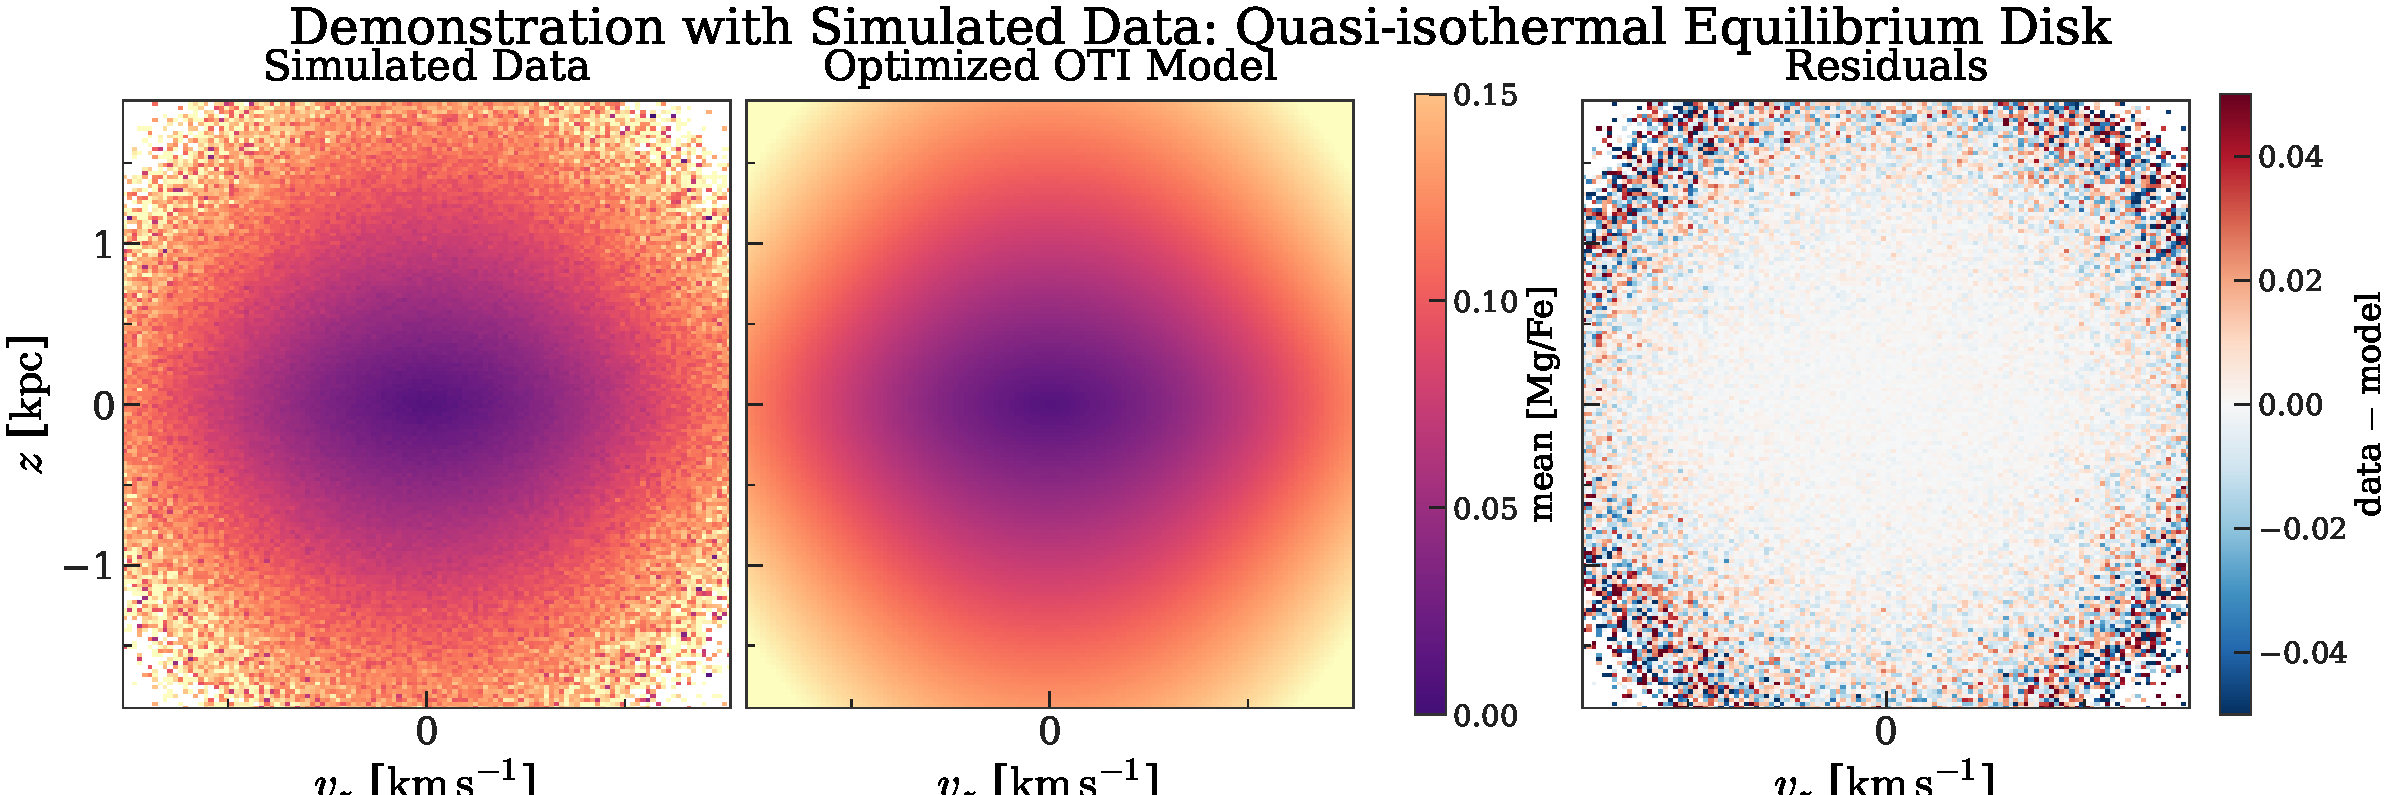
\includegraphics[width=\textwidth]{qiso-data-model.pdf}
\end{center}
\caption{%
The same as Figure~\ref{fig:sho-data-model}, but for the simulated quasi-isothermal disk
sample from Section~\ref{sec:sim-qiso}, showing the simulated data set (left panel), the
optimized OTI model (middle panel), and the residuals (right panel).
% \textbf{Left panel:} Simulated kinematic data in the vertical phase space with an
% isothermal distribution function and a linear relation between \abun{Mg}{Fe} and
% $z_{\textrm{max}}$ (see Figure~\ref{fig:mgfe-zvz}).
% \textbf{Middle panel:} An optimized OTI model evaluated on the same grid of phase-space
% coordinates as the data (left panel).
% \textbf{Right panel:} The residuals of the best-fit model (i.e. the simulated data minus
% the best-fit model evaluated on the same grid of phase-space coordinates).
\label{fig:qiso-data-model}
}
\end{figure*}

\begin{figure*}[t!]
\begin{center}
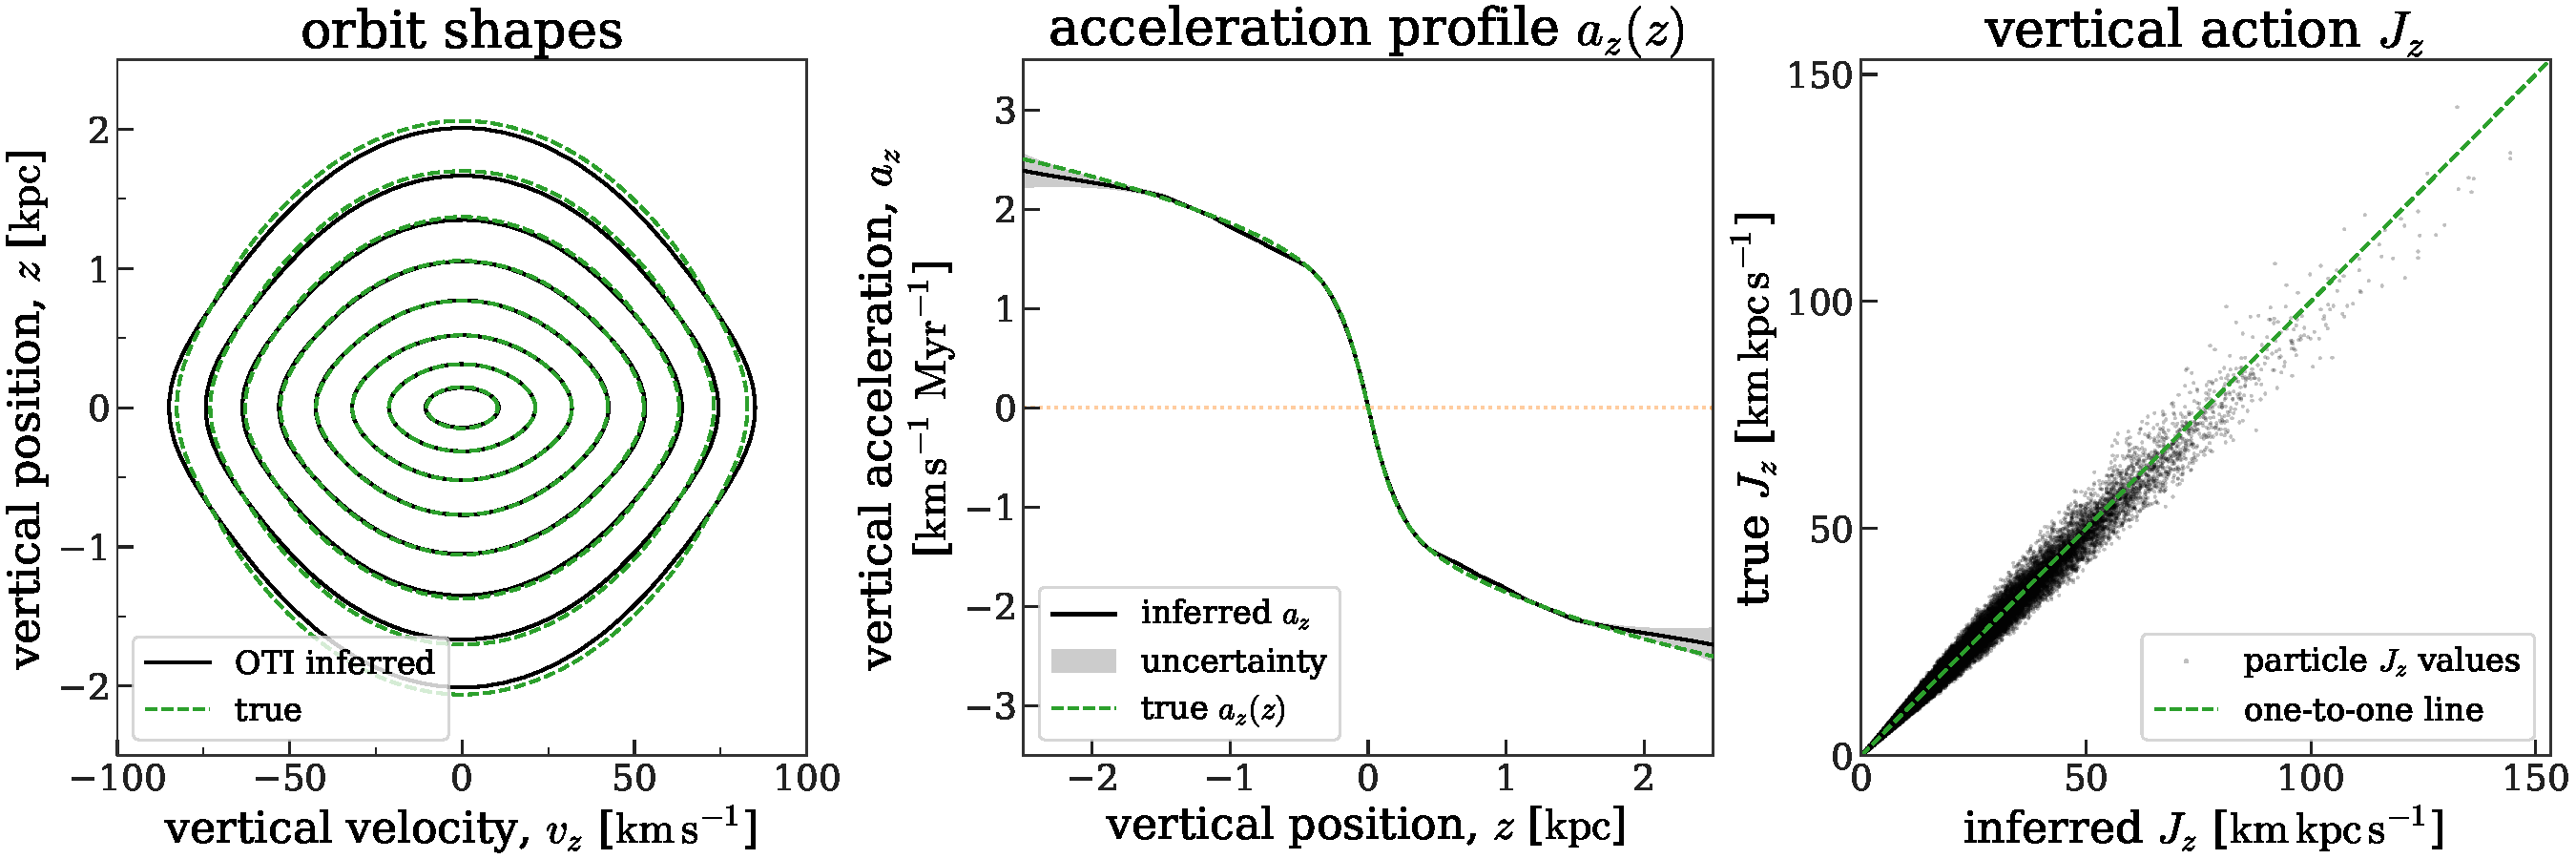
\includegraphics[width=\textwidth]{qiso-validation.pdf}
\end{center}
\caption{%
Validation of the OTI model fit to the simulated quasi-isothermal disk sample. (i.e. the
same as Figure~\ref{fig:sho-validation}, but for the simulated disk sample from
Section~\ref{sec:sim-qiso}).
\todo{Audit fractional error}
The median (fractional) action error is $\approx 4\%$ for this sample dataset, but we do
not need to assume a gravitational potential to compute the actions.
\label{fig:qiso-validation}
}
\end{figure*}

\subsection{Axisymmetric Quasi-isothermal Disk with Survey Selection}
\label{sec:sim-qiso-sel}

Real data from stellar surveys often has complex selection effects resulting from survey
targeting and design, instrument limitations (e.g., magnitude limits), and/or real
astronomical effects like bright stars, crowding, or dust extinction.
All of these effects predominantly depend on position and brightness of the sources
considered and not strongly on derived parameters like element abundances.
One of the benefits of OTI is that positional

\begin{figure*}[t!]
\begin{center}
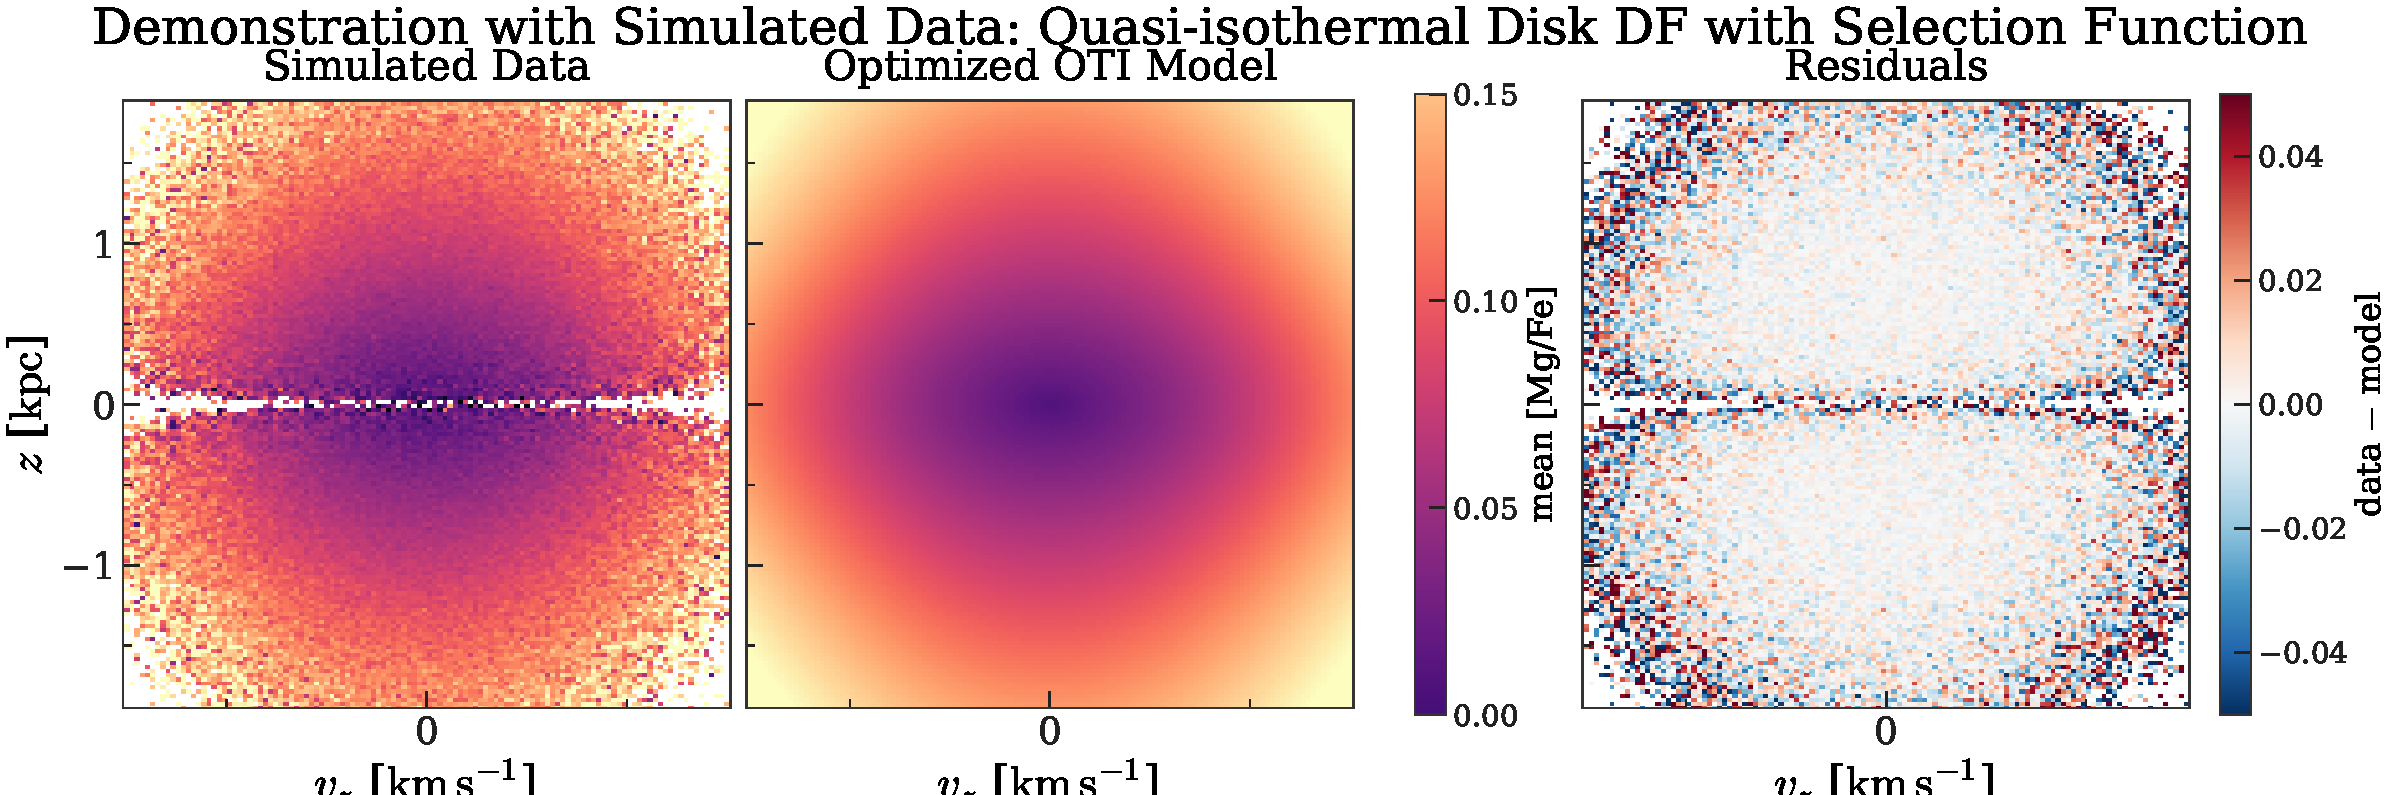
\includegraphics[width=\textwidth]{qiso-sel-data-model.pdf}
\end{center}
\caption{%
The same as Figure~\ref{fig:sho-data-model}, but for the simulated quasi-isothermal disk
sample from Section~\ref{sec:sim-qiso}, showing the simulated data set (left panel), the
optimized OTI model (middle panel), and the residuals (right panel).
\label{fig:qiso-sel-data-model}
}
\end{figure*}


\subsection{N-body Simulation with a Perturbed Disk}
\label{sec:sim-jason}

As a final demonstration, we apply the OTI framework to a section of an N-body simulation of a stellar disk that has been perturbed by an orbiting satellite galaxy. 

For this, we use the $N$-body simulation M1 of the \texttt{SMUDGE}\ simulation suite \cite{Hunt:2021} now available on \texttt{SciServer}\footnote{https://sciserver.org/datasets/smudge/} \citep{sciserver}. M1 simulates the merger of a $\sim8\times10^{10}$ M$_{\odot}$ dwarf galaxy consisting of two Hernquist spheres \citep{Hernquist:1990} into a $\sim6\times10^{11}$ $M_{\odot}$ disc galaxy host. The host galaxy consists of a $8.8\times10^8$ particle live NFW halo \citep{Navarro:1997}, a $2.2\times10^7$ particle Hernquist bulge and a $2.2\times10^8$ particle exponential disc with a high Toomre parameter $\mathcal{Q}=2.2$ \citep{Toomre:1964}, following model MWb from \cite{Widrow:2005}. For full details of the initial condition and simulation setup see \cite{Hunt:2021}.

The merger simulation is evolved for $\sim8.3$ Gyr using the GPU based $N$-body tree code, \texttt{Bonsai}\ \citep{Bedorf:2012,Bedorf:2014}. Following \cite{Hunt:2021} we choose snapshot 702 (occurring at $t=6.874$) as the `present day' snapshot used in this work, as this is the snapshot where satellite is closest to the location of the Sagittarius dwarf galaxy in the Milky Way. However, we stress that model M1 is not meant to reproduce the Milky Way - Sagittarius interaction \citep[instead see][]{Bennett:2022} but instead be a laboratory for exploring satellite induced perturbation in an otherwise stable disc.

\todo{Jason - can you help fill in a few sentences about the simulation here and read below to make sure I say correct things!}
The simulation ... describe it ...

We use a snapshot of the simulation after four pericentric passages, and six disc crossings of the
satellite \citep[see Figure 3 of][for the orbit and mass loss of the satellite]{Hunt:2021}, which induces significant non-axisymmetric kinematic structure in the disk.
Figure~\ref{fig:jason-mean-z-vz} shows the mean vertical position (left panel) and
vertical velocity (right panel) of stars across the face of the simulated disk, showing
that the disk is rich with substructure as a result of repeat satellite perturbations.
This application is a test of how well OTI can do (i.e. how biased the results are) in
the presence of strong disequilibrium, which violates the assumptions laid out above.

We select a small region of the disk near the solar radius, $R=8~\kpc$, by selecting all
star particles within $|x-8~\kpc| < 1.5~\kpc$ and $|y| < 1.5~\kpc$.
We again mimic dynamical selections we could perform on real data by selecting stars
near their guiding-center radius $R_G$, i.e. $|R-R_G| < 1~\kpc$, and with small radial
velocity $|v_R| < 15~\kms$.
These dynamical selections limit the radial action of the stars so that our assumption
of $R$--$z$ separability is less invalid, but does not require computing actions for the
star particles before selection.
We compute the guiding radii using the circular velocity curve of the simulated disk,
$R_G \approx L_z / v_c(R)$, but here we use actions only to select a sample of stars on
nearly circular orbits with which to measure the circular velocity.
We compute the circular velocity by selecting star particles with low radial and
vertical action (below the 15th percentile values of the radial and vertical actions,
respectively) and compute the mean azimuthal velocity $\langle v_\phi(R) \rangle$ as a
function of cylindrical radius $R$, then adopt $v_c(R) = \langle v_\phi(R) \rangle$.
\todo{Jason - describe how the actions were computed}
The actions are computed using \texttt{Agama}\ \citep{Vasiliev:2019}. We first approximate the host galaxy potential using two multipole expansions for the stellar bulge and dark matter halo, and an axisymmetric \texttt{CylSpline}\ expansion for the disc. We calculate actions, angles and frequencies in the reconstructed potential using \texttt{Agama}'s \texttt{ActionFinder}\ routine.

We also use the orbital actions to ``paint'' element abundances onto star particles in
this idealized $N$-body simulation without gas or star formation.
We compute the actions at an early snapshot of the simulation, after relaxation of the
initial conditions and before the first pericentric passage of the satellite galaxy.
We use the vertical actions of the star particles at this early snapshot to assign a
simulated \abun{Mg}{Fe} abundance value to each star particle following the procedure
explained in Section~\ref{sec:sim-qiso}.
We then track the abundance values through to the final snapshot where the actions have
evolved due to satellite perturbations.

Figure~\ref{fig:jason-data-model} (left panel) shows the mean simulated \abun{Mg}{Fe}
abundance of star particles in the vertical phase space of the ``solar neighborhood'' of
the simulated stellar disk.
While the overall pattern is similar to the smooth examples (e.g.,
Section~\ref{sec:sim-qiso}), the mean abundance values here show an appreciable ``phase
spiral'' akin to the vertical phase-space spiral seen in kinematics alone
\citep{Antoja:2018}.
The middle panel of Figure~\ref{fig:jason-data-model} shows the mean \abun{Mg}{Fe} of
the optimized OTI model for this simulated data set, and the right panel again shows the
residuals.
While the residuals are generally low, the simulated abundance spiral is faintly visible
here in the residuals, which may bias our inferred dynamical quantities.

Figure~\ref{fig:jason-validation} (left panel) shows the vertical acceleration profile
inferred by OTI for this region of the simulated disk (black line and gray shaded
region) compared to the true acceleration profile.
The right panel of Figure~\ref{fig:jason-validation} shows a comparison of vertical
action values computed with the best-fit OTI model (horizontal axis) and with Agama
(vertical axis).
The actions computed with Agama are not necessarily ``true'' values, as this system is
not in equilibrium or symmetric, but the adopted potential model used to compute the
actions is both axisymmetric and time-invariant.
At $z=1~\kpc$, we find ... TODO




\section{Applications to Data} \label{sec:applications-data}

In this section, we apply the OTI framework to data from the \apogee\ surveys and \gaia\
Data Release 3.
In Section~\ref{sec:apogee}, we fit the mean \abun{Mg}{Fe} data shown in
Figure~\ref{fig:mgfe-zvz} to infer the vertical acceleration profile at the solar
radius.
However, we consider this to be a limited demonstration, as a full analysis of the
\apogee\ data is presented in a companion paper \citep{Horta:2023}.
In Section~\ref{sec:gaiadr3}, we use the vertical kinematics alone (using phase-space
data from \gaia) to demonstrate using the phase-space density itself as a stellar label.
We additionally show how OTI is useful as a means to fit a flexible but symmetric model
of the phase space to subtract and reveal the residuals, which provides a new means to
characterize the vertical phase-space spirals around the Milky Way.

\subsection{Data sources} \label{sec:data}

\todo{standard blurbs about APOGEE and Gaia}


\subsection{The vertical \abun{Mg}{Fe} gradient in the solar neighborhood with \apogee}
\label{sec:apogee}

TODO


\subsection{The local vertical phase space in \gaia\ Data Release 3}
\label{sec:gaiadr3}

TODO: Empirical actions - show frequency-theta with empirical

Fit the vertical acceleration in a slice around the sun, ignoring selection function.
Show residuals: Phase spiral-o-rama

Also compute empirical actions and compare to Agama.


\section{Discussion} \label{sec:discussion}

Limitation that our acceleration can depend on $v_z$.




\section{Summary and Conclusions} \label{sec:conclusions}


\begin{acknowledgements}

It is a pleasure to thank ...

% Funding for the Sloan Digital Sky Survey IV has been provided by the Alfred P.
% Sloan Foundation, the U.S. Department of Energy Office of Science, and the
% Participating Institutions. SDSS-IV acknowledges support and resources from the
% Center for High-Performance Computing at the University of Utah. The SDSS web
% site is www.sdss.org.

% SDSS-IV is managed by the Astrophysical Research Consortium for the
% Participating Institutions of the SDSS Collaboration including the Brazilian
% Participation Group, the Carnegie Institution for Science, Carnegie Mellon
% University, the Chilean Participation Group, the French Participation Group,
% Harvard-Smithsonian Center for Astrophysics, Instituto de Astrof\'isica de
% Canarias, The Johns Hopkins University, Kavli Institute for the Physics and
% Mathematics of the Universe (IPMU) / University of Tokyo, Lawrence Berkeley
% National Laboratory, Leibniz Institut f\"ur Astrophysik Potsdam (AIP),
% Max-Planck-Institut f\"ur Astronomie (MPIA Heidelberg), Max-Planck-Institut
% f\"ur Astrophysik (MPA Garching), Max-Planck-Institut f\"ur Extraterrestrische
% Physik (MPE), National Astronomical Observatories of China, New Mexico State
% University, New York University, University of Notre Dame, Observat\'ario
% Nacional / MCTI, The Ohio State University, Pennsylvania State University,
% Shanghai Astronomical Observatory, United Kingdom Participation Group,
% Universidad Nacional Aut\'onoma de M\'exico, University of Arizona, University
% of Colorado Boulder, University of Oxford, University of Portsmouth, University
% of Utah, University of Virginia, University of Washington, University of
% Wisconsin, Vanderbilt University, and Yale University.

This work has made use of data from the European Space Agency (ESA) mission
{\it Gaia} (\url{https://www.cosmos.esa.int/gaia}), processed by the {\it Gaia}
Data Processing and Analysis Consortium (DPAC,
\url{https://www.cosmos.esa.int/web/gaia/dpac/consortium}). Funding for the DPAC
has been provided by national institutions, in particular the institutions
participating in the {\it Gaia} Multilateral Agreement.

\end{acknowledgements}

\software{
    Astropy \citep{astropy:2013, astropy:2018, astropy:2022},
    gala \citep{gala},
    IPython \citep{ipython},
    numpy \citep{numpy},
    % pymc3 \citep{Salvatier2016},
    % schwimmbad \citep{schwimmbad:2017},
    scipy \citep{scipy}.
}

\appendix

\section{A Toy Milky Way Mass Model}
\label{sec:appendix-potential}

TODO


\section{Monotonic Quadratic Spline}
\label{sec:appendix-spline}

TODO

\section{Evaluation of the Vertical Acceleration from an OTI Model}
\label{sec:appendix-az}

We would like to evaluate the vertical acceleration as a function of height above the
Galactic midplane, $a_z(z) = \frac{\partial \Phi}{\partial z}$.
From the collisionless Boltzmann equation (Equation~\ref{eq:cbe-1d}), after rearranging
terms, we have:
\begin{align}
    \frac{\partial \Phi}{\partial z} &=
        v_z \, \frac{\partial f}{\partial z} \,
        \left( \frac{\partial f}{\partial v_z} \right)^{-1} \\
    &= v_z \, \frac{\partial f}{\partial \rz} \, \frac{\partial \rz}{\partial z} \,
        \left( \frac{\partial f}{\partial \rz} \frac{\partial \rz}{\partial v_z} \right)^{-1} \\
        &= v_z \, \frac{\partial \rz}{\partial z} \,
        \left( \frac{\partial \rz}{\partial v_z} \right)^{-1}
\end{align}
The acceleration only depends on the shapes of the contours of the DF, i.e. curves of
constant \rz, so that we only need to differentiate the distorted radius to evaluate it.
Recall that, based on our definitions above,
\begin{align}
    \rzp &= \sqrt{z^2 \, \freqzero + v_z^2 \, \freqzero^{-1}} \\
    \thzp &= \tan^{-1}\left(\frac{z}{v_z} \, \freqzero\right) \\
    \rz &= \rzp \, \left( 1 + \sum_{m=2}^{\mmax} e_m(\rzp) \,
        \cos(m \, \thzp) \right) \label{eq:rz-rzp}
\end{align}
where the sum in Equation~\ref{eq:rz-rzp} is only over even values of $m$.

We must compute the partial derivatives of \rz\ with respect to $z$ and $v_z$:
\begin{align}
    \frac{\partial \rz}{\partial z} &=
        \frac{\partial \rzp}{\partial z} +
        \sum_{m=2}^{\mmax} \frac{\partial}{\partial z} \left[\rzp \, e_m(\rzp) \, \cos\left(m \, \thzp\right)\right]\\
    \frac{\partial \rz}{\partial v_z} &=
        \frac{\partial \rzp}{\partial v_z} +
        \sum_{m=2}^{\mmax} \frac{\partial}{\partial v_z} \left[\rzp \, e_m(\rzp) \, \cos\left(m \, \thzp\right)\right]
\end{align}

To work out the resulting expressions, we will make use of the following terms:
\begin{alignat}{3}
    \frac{\partial \rzp}{\partial z} &= \frac{z\,\freqzero}{\rzp} \quad &; \quad
        \frac{\partial \rzp}{\partial v_z} &= \frac{v_z}{\freqzero \, \rzp} \\
    \frac{\partial \thzp}{\partial z} &= \frac{v_z}{\rzp^2} \quad &; \quad
        \frac{\partial \thzp}{\partial v_z} &= -\frac{z}{\rzp^2} \\
    \frac{\partial e_m}{\partial z} &=
        \frac{\partial e_m}{\partial \rzp} \, \frac{\partial \rzp}{\partial z}
        \quad &; \quad
        \frac{\partial e_m}{\partial v_z} &=
        \frac{\partial e_m}{\partial \rzp} \, \frac{\partial \rzp}{\partial v_z}
\end{alignat}

Our goal is to remove or collect terms that explicitly contain $v_z$, as we are going to
take the limit as $\thzp \to \frac{\pi}{2}$, i.e. to evaluate the acceleration along the
$z$-axis, which implies $v_z \to 0$.
Starting with the derivative with respect to $z$:
\begin{align}
    \frac{\partial \rz}{\partial z} &=
        \frac{\partial \rzp}{\partial z} +
        \sum_{m=2}^{\mmax} \frac{\partial}{\partial z}
            \left[\rzp \, e_m(\rzp) \, \cos(m \, \thzp)\right]\\
    &= \frac{\partial \rzp}{\partial z} +
        \sum_{m=2}^{\mmax} \left[
        \frac{\partial \rzp}{\partial z} \, e_m \, \cos(m \, \thzp)
        + \rzp \, \frac{\partial e_m}{\partial z} \, \cos(m \, \thzp)
        - \rzp \, e_m \, \sin(m \, \thzp) \, m \,\frac{\partial \thzp}{\partial z}\right]\\
    &= \frac{z\,\freqzero}{\rzp} + \sum_{m=2}^{\mmax} \left[
        \frac{z\,\freqzero}{\rzp} \, e_m \, \cos(m \, \thzp) +
        \rzp \, \frac{z\,\freqzero}{\rzp} \, \frac{\partial e_m}{\partial \rzp} \, \cos(m \, \thzp) -
        \rzp \, e_m \, \sin(m \, \thzp) \, m \, \frac{v_z}{\rzp^2}\right]\\
    &= \frac{z\,\freqzero}{\rzp} \, \left[
        1 + \sum_{m=2}^{\mmax} \left(
            e_m \, \cos(m \, \thzp) +
                \rzp \, \frac{\partial e_m}{\partial \rzp} \, \cos(m \, \thzp) -
                m \, e_m \, \sin(m \, \thzp) \, \frac{v_z}{z\,\freqzero}
        \right)
    \right]\\
    &= \frac{z\,\freqzero}{\rzp} \, \left[
        1 + \sum_{m=2}^{\mmax} \left(
            \left(e_m + \rzp \, \frac{\partial e_m}{\partial \rzp}\right) \,
                \cos(m \, \thzp) -
            m \, e_m \, \frac{\sin(m \, \thzp)}{\sin(\thzp)} \, \cos(\thzp)
        \right)
    \right]
\end{align}
As we are interested in evaluating this expression along the $z$-axis, we will take the
limit of this expression as $\thzp \to \frac{\pi}{2}$.
For even values of $m$, as we require, the sine term in the sum will be zero, and the
cosine terms become:
\begin{equation}
    \cos(m \, \thzp) = (-1)^{m/2} \quad .
\end{equation}
In this limit, the expression becomes:
\begin{equation}
    \lim_{\thzp \to \frac{\pi}{2}} \frac{\partial \rz}{\partial z} =
        \frac{z\,\freqzero}{\rzp} \, \left[
            1 + \sum_{m=2}^{\mmax} (-1)^{m/2} \,
                \left(e_m + \rzp \, \frac{\partial e_m}{\partial \rzp}\right)
        \right] \quad .
\end{equation}

Similarly for the derivative with respect to $v_z$:
\begin{align}
    \frac{\partial \rz}{\partial v_z} &=
        \frac{\partial \rzp}{\partial v_z} +
        \sum_{m=2}^{\mmax} \frac{\partial}{\partial v_z}
            \left[\rzp \, e_m(\rzp) \, \cos(m \, \thzp)\right]\\
    &= \frac{\partial \rzp}{\partial v_z} +
        \sum_{m=2}^{\mmax} \left[
        \frac{\partial \rzp}{\partial v_z} \, e_m \, \cos(m \, \thzp)
        + \rzp \, \frac{\partial e_m}{\partial v_z} \, \cos(m \, \thzp)
        - \rzp \, e_m \, \sin(m \, \thzp) \, m \,\frac{\partial \thzp}{\partial v_z}\right]\\
    &= \frac{v_z}{\freqzero\,\rzp} + \sum_{m=2}^{\mmax} \left[
        \frac{v_z}{\freqzero\,\rzp} \, e_m \, \cos(m \, \thzp) +
        \rzp \, \frac{v_z}{\freqzero\,\rzp} \, \frac{\partial e_m}{\partial \rzp} \, \cos(m \, \thzp) +
        \rzp \, e_m \, \sin(m \, \thzp) \, m \, \frac{z}{\rzp^2}\right]\\
    &= \frac{v_z}{\freqzero \, \rzp} \, \left[
        1 + \sum_{m=2}^{\mmax} \left(
            e_m \, \cos(m \, \thzp) +
                \rzp \, \frac{\partial e_m}{\partial \rzp} \, \cos(m \, \thzp) +
                m \, e_m \, \sin(m \, \thzp) \, \tan(\thzp)
        \right)
    \right]\\
    &= \frac{v_z}{\freqzero \, \rzp} \, \left[
        1 + \sum_{m=2}^{\mmax} \left(
            \left(e_m + \rzp \, \frac{\partial e_m}{\partial \rzp}\right) \,
                \cos(m \, \thzp) +
            m \, e_m \, \sin(m \, \thzp) \, \tan(\thzp)
        \right)
    \right]
\end{align}
Taking the same limit $\thzp \to \frac{\pi}{2}$, this expression becomes:
\begin{equation}
    \lim_{\thzp \to \frac{\pi}{2}} \frac{\partial \rz}{\partial v_z} =
        \frac{v_z}{\freqzero \, \rzp} \, \left[
            1 + \sum_{m=2}^{\mmax} (-1)^{m/2} \,
                \left(e_m\,(1 - m^2) + \rzp \, \frac{\partial e_m}{\partial \rzp}\right)
        \right] \quad .
\end{equation}

Combining these expressions, we have:
\begin{align}
    \frac{\partial \Phi}{\partial z} &=
        v_z \, \frac{\partial \rz}{\partial z} \,
        \left( \frac{\partial \rz}{\partial v_z} \right)^{-1}\\
    &= v_z \, \frac{z\,\freqzero}{\rzp} \, \frac{\freqzero \, \rzp}{v_z} \,
        \frac{\left[
            1 + \sum_{m=2}^{\mmax} (-1)^{m/2} \,
                \left(e_m + \rzp \, \frac{\partial e_m}{\partial \rzp}\right)
        \right]}{\left[
            1 + \sum_{m=2}^{\mmax} (-1)^{m/2} \,
                \left(e_m\,(1 - m^2) + \rzp \, \frac{\partial e_m}{\partial \rzp}\right)
        \right]} \\
    &= \freqzero^2 \, z \,
        \frac{\left[
            1 + \sum_{m=2}^{\mmax} (-1)^{m/2} \,
                \left(e_m + \rzp \, \frac{\partial e_m}{\partial \rzp}\right)
        \right]}{\left[
            1 + \sum_{m=2}^{\mmax} (-1)^{m/2} \,
                \left(e_m\,(1 - m^2) + \rzp \, \frac{\partial e_m}{\partial \rzp}\right)
        \right]}
\end{align}

\section{Model Function and Parameter Choices}
\label{sec:appendix-params}

TODO: Move all tables down here?

\begin{table}
    \begin{centering}
\begin{tabular}{c c c}
    \multicolumn{3}{c}{\textbf{Simple Harmonic Oscillator Model Fit}} \\ [0.75ex]
    Parameter & Description & Bounds \\ [0.5ex]
    \hline\hline
    $\ln(\freqzero / (\unit{\radian\per\mega\year}))$ & Asymptotic frequency at $r_z=0$ & $(-9, 0)$\\
    $z_0$ & Solar position relative to midplane & $(-0.5, 0.5)~\kpc$\\
    $v_{z,0}$ & Solar velocity relative to midplane & $(-50, 50)~\kms$\\
    $y_0^{\ln n}$ & Label function value (\abun{Mg}{Fe}) at $r_z=0$ & $(-5, 25)$\\
    $y_{1\dots K}^{\ln n}$ & Label function derivative values & $(-25, 0)$\\
    $y_0^{e_2}$ & $m=2$ Fourier coefficient function value at $r_z=0$ & fixed to $0$\\
    $y_{1\dots L}^{e_2}$ & $m=2$ Fourier coefficient function derivative values & $(0, 1)$\\
\end{tabular}
\caption{
    A summary of the parameters and parameter bounds used for fitting the simulated
    simple harmonic oscillator data in Section~\ref{sec:sim-sho}.
    We use $K=10$ spline knots for the log-phase-space density spline function and $L=5$
    spline knots for the $m=2$ Fourier coefficient spline function.
    In total, this model has 17 free parameters.
    \label{tbl:sho-params}
}
\end{centering}
\end{table}

% TODO: update the table
\begin{table}
    \begin{centering}
\begin{tabular}{c c c}
    \multicolumn{3}{c}{\textbf{Quasi-isothermal Disk Model Fit}} \\ [0.75ex]
    Parameter & Description & Bounds \\ [0.5ex]
    \hline\hline
    $\ln(\freqzero / (\unit{\radian\per\mega\year}))$ & Asymptotic frequency at $r_z=0$ & $(-9, 0)$\\
    $z_0$ & Solar position relative to midplane & $(-0.5, 0.5)~\kpc$\\
    $v_{z,0}$ & Solar velocity relative to midplane & $(-50, 50)~\kms$\\
    $y_0^{\ln n}$ & Label function value (\abun{Mg}{Fe}) at $r_z=0$ & $(-5, 25)$\\
    $y_{1\dots K}^{\ln n}$ & Label function derivative values & $(-25, 0)$\\
    $y_0^{e_2}$ & $m=2$ Fourier coefficient function value at $r_z=0$ & fixed to $0$\\
    $y_{1\dots L}^{e_2}$ & $m=2$ Fourier coefficient function derivative values & $(0, 1)$\\
\end{tabular}
\caption{
    A summary of the parameters and parameter bounds used for fitting the simulated
    simple harmonic oscillator data in Section~\ref{sec:sim-sho}.
    We use $K=10$ spline knots for the log-phase-space density spline function and $L=5$
    spline knots for the $m=2$ Fourier coefficient spline function.
    In total, this model has 17 free parameters.
    \label{tbl:sho-params}
}
\end{centering}
\end{table}

\bibliographystyle{aasjournal}
\bibliography{refs}

\end{document}

% % Context
% In a steady-state dynamical system, spatial gradients of the phase-space density (the
% distribution function, \df) of any tracers are related to gradients of the underlying
% gravitational potential (the acceleration field).
% This is the basis of many methods used in Galactic dynamics to infer the mass or dark
% matter distribution of the Milky Way, often with highly-symmetric, few-component,
% parametric models of the Galaxy (e.g., an exponential disk with constant scale height).
% However, we know that the Galaxy is not in equilibrium and its mass distribution is
% complex:
% Stellar kinematics show signatures of non-steady-state dynamics throughout the Galactic
% disk and significant departures from axisymmetry.
% % Aims
% We aim to develop a framework for measuring the acceleration field of the Milky Way, in
% the presence of weak disequilibrium, that makes few assumptions about the form of the
% mass distribution.
% % Methods
% Here we outline a flexible method for empirically modeling the vertical phase-space
% density (or mean statistics of stellar invariants in this phase-space, like element
% abundances) of stars in the Galactic disk.
% This method --- an improved version of the method of \emph{Orbital Torus Imaging} (OTI)
% --- works by exploiting the fact that orbital trajectories in the vertical phase-space
% of an unperturbed galaxy have predictable symmetries in projections of phase-space and
% can be represented as a low-order Fourier expansion away from an ellipse.
% % Results
% We first demonstrate OTI using a toy simulation of a vertical phase-space distribution
% of stars, then with a more realistic galactic disk population, and show that in both
% cases OTI recovers the local vertical acceleration as a function of height above the
% galactic midplane.
% We then show that this method enables us to compute \emph{empirical} orbital actions,
% angles, and frequencies for stars where the approximation of a separable 1D phase-space
% is valid: This enables interpreting the timescales of disequilibrium features in a
% flexible way that does not require adopting a global model of the gravitational
% potential.
% For example, we demonstrate that this method provides a useful tool for studying the
% \emph{residuals} away from an equilibrium model, such as the ``\gaia\ Phase Spiral.''
% % Conclusions
% Some conclusions.

% Context
% Orbital dynamics is complex in six-dimensional phase-space, making it a challenge to
% interpret the rich and structured kinematic data of stars in the Milky Way revealed in
% recent data releases from the \gaia\ Mission.
% In a symmetric, steady-state galaxy, or in the presence of only weak perturbations, the
% dynamical interpretation and investigation of kinematic data is often simplified by
% using dynamical invariants such as orbital actions.
% However, computing many such quantities (e.g., the energy, actions, fundamental
% frequencies, etc.) require having a model for the gravitational potential and, even so,
% are either slow to compute or imprecise.
% % Aims
% To mitigate at least one of these limitations, we aim to demonstrate a method for
% estimating fundamental galactic orbital properties for stars directly from the kinematic
% and stellar label data (e.g., element abundances) without requiring a gravitational
% potential model.
% % Methods
% This method still assumes a symmetric and steady-state distribution function, but uses
% either the number density of stars in a slice of phase-space (e.g., vertical $z$--$v_z$
% kinematics) or a statistic computed from other stellar invariants in this slice (e.g.,
% element abundances) to empirically estimate orbital actions, frequencies, and angles for
% the stars.
% % Results
% We demonstrate the method using a toy equilibrium model where orbital properties are
% known, and then show applications of this method even in the presence of disequilibrium.
% As a last demonstration, we use data from the \gaia\ Mission to estimate the total mass
% density at the Galactic midplane as a function of radius near the sun.
% % Conclusions
% We conclude :shrugs:.


% The fundamental objects of a statistical approach to Galactic dynamics are the tracer
% distribution function (DF), $f(\bs{x}, \bs{v}, t)$, which describes the probability of
% observing a star at position $\bs{x}$ and velocity $\bs{v}$ at time $t$, and the total
% gravitational potential, $\Phi(\bs{x}, t)$, which is related to the mass density
% distribution we seek $\rho(\bs{x}, t)$ through Poisson's equation $\nabla^2 \Phi =
% 4\pi G \, \rho$. Many dynamical inference methods have been built to connect these two
% objects (the DF and the potential) in order to measure properties of the mass
% distribution of the Milky Way and other galaxies (CITE). These methods can be broadly
% categorized into two classes: those that work with gradients of the DF to measure
% gradients of the potential (CITE), or those that model the form of the DF itself
% (CITE). In either case, the majority of applications of these methods have assumed
% that the Galaxy is in equilibrium and the DF is in steady state so that the explicit
% time dependence of the DF and potential can be ignored. Most applications also assume
% that the DF and potential are separable in some coordinates (for example, cylindrical
% radius $R$ and height $z$, for disk modeling), and that the DF and/or potential can be
% expressed by a set of smooth, parametric model terms for which the parameters can be
% inferred from the data. These methods and assumptions have enabled a wide array of
% measurements of the structure and mass distribution of the Milky Way's disk, central
% region, stellar halo, and dark matter content over the last century (CITE).


% However, the current data volume and precision presents a challenge to current and
% past dynamical inference methods that make use of stellar kinematics. Many of these
% methods rely on assumptions that are violated at very high signal-to-noise ratio ---
% that is, the principle ``challenge'' of utilizing modern stellar kinematic data is
% that large surveys have revealed the complexity of the Milky Way at high significance.
% For example, the observed DF of stars in the Milky Way disk is highly sub-structured
% on small and large-scales in phase-space. This includes local features like the \gaia\
% ``phase spiral'' in the vertical kinematics of stars (CITE), or the historically-named
% ``moving groups'' in the in-plane kinematics or integrals of motions (CITE Trick,
% Hunt, etc.). But this also includes large-scale features like ``ridges'' in the
% vertical velocity as a function of Galactic radius (CITE), an overall warp and flaring
% of the disk (CITE), and significant bulk motion of stars in their in-plane velocities
% (CITE Katz, Eilers), to name a few. These features of the DF suggest that the
% underlying mass distribution or gravitational potential is significantly time
% dependent. With historical data volumes and precision, these things could be ignored
% and averaged over because the signatures were subtle. However, with the quality and
% volume of data at present, ignoring these features (which appear in most phase-space
% dimensions as deviations from steady-state at the 10--50\% level; CITE) will produce
% very precise but biased measurements about the Milky Way and its dark matter.

% To study signatures of disequilibrium and non-steady-state features in the DF, there
% has been significant effort in using equilibrium models as a means to subtract a
% smooth model from the data and thereby reveal the underlying substructure and
% deviations from equilibrium (CITE). This has enabled tracing features like the \gaia\
% phase spiral throughout the Milky Way disk (CITE) and in stellar invariants like
% element abundances (CITE Neige). However, to \emph{model} or fit these non-equilibrium
% features, there is no universal framework for doing this. One approach to dealing with
% the observed complexity of the stellar kinematics in the Milky Way is to build
% explicit parametric model components of the DF and potential to account for all time
% dependence of both. In principle, with flexible enough parametrizations, this should
% work fine to produce unbiased measurements of the potential and therefore the dark
% matter and mass distribution of the Galaxy. However, this requires making decisions
% about how to parametrize the time dependence, which could be arbitrarily complex.

% With the present data volumes and precisions, which lead to incredibly precise
% parameter constraints, these decisions can easily lead to biased model fits. This
% motivates developing flexible dynamical inference methods that make fewer explicit
% assumptions about the potential and DF. Conceptually, we imagine developing new
% methods that can separate the tasks of ``fitting the data'' and ``interpreting the
% model fits in terms of dynamics.'' The benefit of this approach is that, by releasing
% both in any study of stellar kinematics, subsequent work can build on the
% interpretation without having to rebuild the data analysis aspects of the method.

% Another major motivator for thinking about new methods is that many stellar surveys
% deliver stellar parameters and element abundances alongside kinematic measurements.
